\cotefile{148}

\scanpage{21}

\figure{\begin{tikzpicture}[x=0.009cm,y=-0.009cm,line cap=round,line join=round]
% The short isolated strokes and the six long strokes around the sketches.
\draw[line width=.65pt] (222,143)..controls(245,131)and(261,132)..(289,149);
\draw[gray!65,line width=.35pt] (392,493)..controls(403,480)and(405,468)..(427,461);
\draw[gray!65,line width=.4pt] (800,94)..controls(789,88)and(788,179)..(792,260)..controls(790,319)and(789,367)..(799,382)..controls(808,373)and(808,362)..(805,337)..controls(802,251)and(810,137)..(800,94);
\draw[gray!65,line width=.4pt] (395,230)..controls(475,303)and(552,387)..(653,501);
\draw[gray!65,line width=.4pt] (1047,387)..controls(1106,337)and(1169,259)..(1192,242)--(1210,231);
\draw[gray!65,line width=.4pt] (348,773)..controls(431,717)and(525,651)..(597,595);
\draw[gray!65,line width=.4pt] (759,688)..controls(764,781)and(750,905)..(756,1000);
\draw[gray!65,line width=.4pt] (866,624)..controls(940,675)and(1011,757)..(1086,805);

% The larger sketch: five solid edges and one edge in six visible dashes.
\draw[line width=.8pt] (665,574)..controls(705,521)and(739,469)..(769,432)..controls(790,458)and(827,499)..(852,527);
\draw[line width=.8pt] (856,533)--(802,617);
\draw[line width=.55pt] (666,575)..controls(712,592)and(762,615)..(795,621);
\draw[line width=.9pt] (770,435)..controls(778,506)and(790,566)..(801,616);
\draw[gray!75,line width=.4pt] (667,569)--(762,440);
\draw[line width=.6pt] (674,568)--(696,561) (704,557)--(723,553) (732,551)--(744,549) (755,545)--(769,540) (788,540)--(801,537) (816,535)--(847,530);

% The smaller sketch and its superposed oblique strokes; no labels occur.
\draw[gray!80,line width=.45pt] (918,469)--(991,347)..controls(1008,365)and(1047,391)..(1075,404);
\draw[gray!80,line width=.45pt] (1083,418)--(1035,497)--(919,471);
\draw[gray!80,line width=.45pt] (991,351)--(1036,497) (920,468)--(1077,416);
\draw[gray!60,line width=.35pt] (922,474)--(988,354) (1038,491)--(1085,418) (1029,475)--(1023,438);
\draw[gray!70,line width=.55pt] (916,509)--(1048,389);
% The dark diagonal is copied as separate visible strokes, without an inferred arrowhead.
\draw[line width=.75pt] (969,483)--(987,462) (997,449)--(1012,427) (1017,418)--(1045,392);
\draw[line width=.55pt] (1001,444)--(1033,408);
\draw[line width=.55pt] (1004,405)..controls(1014,399)and(1019,397)..(1025,399);
\end{tikzpicture}}

\margin{20}

\scanpage{22}

\texttt{//* GUTS 0055 I}

\figure{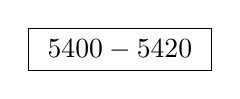
\begin{tikzpicture}
\node[draw,inner xsep=7pt,inner ysep=4pt] {$5400-5420$};
\end{tikzpicture}}

\margin{\handwritten{(93) 51, 81, 00 \quad 411.}}

\figure{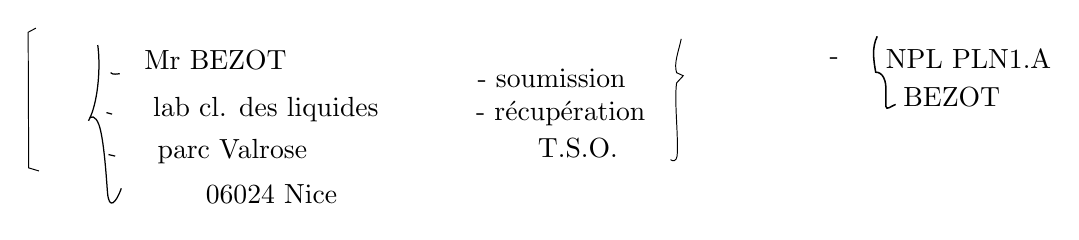
\begin{tikzpicture}[x=0.0065cm,y=-0.0065cm,
  every node/.style={anchor=west,inner sep=0pt,font=\normalsize}]
% The outer brackets finish above the postcode; the inner brace continues down to it.
\draw[line width=0.35pt] (38,9) -- (23,17) -- (24,282) -- (44,288);
\draw[line width=0.35pt] (1299,30) .. controls (1294,54) and (1284,78) .. (1290,96)
  -- (1303,102) -- (1290,116) .. controls (1285,151) and (1294,222) .. (1291,259)
  .. controls (1289,270) and (1283,269) .. (1278,266);
\draw[line width=0.45pt] (159,42) .. controls (165,87) and (159,147) .. (146,179)
  -- (141,190) .. controls (145,177) and (155,181) .. (161,197)
  .. controls (171,223) and (176,304) .. (178,330)
  .. controls (181,366) and (195,350) .. (205,322);
% Three short strokes at the left of the address lines, kept as drawn marks.
\draw[line width=0.45pt] (184,96) .. controls (190,101) and (196,98) .. (202,98);
\draw[line width=0.45pt] (176,174) -- (187,177);
\draw[line width=0.45pt] (180,256) -- (193,259);
\node at (249,72) {\handwritten{Mr BEZOT}};
\node at (266,168) {\handwritten{lab cl. des liquides}};
\node at (275,251) {\handwritten{parc Valrose}};
\node at (369,333) {\handwritten{06024 Nice}};
\node at (900,107) {\handwritten{- soumission}};
\node at (897,176) {\handwritten{- récupération}};
\node at (1018,244) {\handwritten{T.S.O.}};
\node at (1588,69) {\handwritten{-}};
\draw[line width=0.55pt] (1682,25) .. controls (1671,47) and (1675,72) .. (1679,95)
  .. controls (1693,95) and (1700,111) .. (1699,133)
  -- (1699,162) .. controls (1700,170) and (1708,162) .. (1718,158);
\node at (1698,69) {\handwritten{NPL PLN1.A}};
\node at (1732,143) {\handwritten{BEZOT}};
\end{tikzpicture}}

\figure{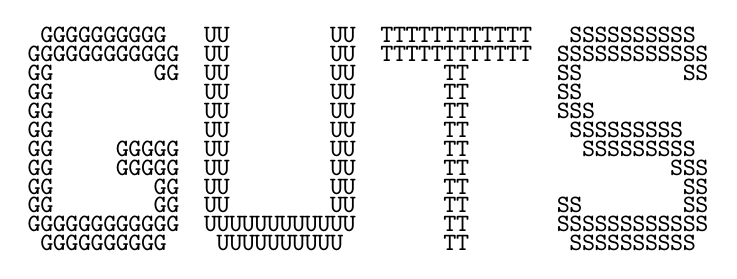
\begin{tikzpicture}[x=0.16cm,y=-0.24cm,
 every node/.style={inner sep=0pt,font=\ttfamily\small}]
\foreach \x/\y in {1/0,2/0,3/0,4/0,5/0,6/0,7/0,8/0,9/0,10/0,0/1,1/1,2/1,3/1,4/1,5/1,6/1,7/1,8/1,9/1,10/1,11/1,0/2,1/2,10/2,11/2,0/3,1/3,0/4,1/4,0/5,1/5,0/6,1/6,7/6,8/6,9/6,10/6,11/6,0/7,1/7,7/7,8/7,9/7,10/7,11/7,0/8,1/8,10/8,11/8,0/9,1/9,10/9,11/9,0/10,1/10,2/10,3/10,4/10,5/10,6/10,7/10,8/10,9/10,10/10,11/10,1/11,2/11,3/11,4/11,5/11,6/11,7/11,8/11,9/11,10/11}
  {\node at (\x,\y) {G};}
\foreach \x/\y in {14/0,15/0,24/0,25/0,14/1,15/1,24/1,25/1,14/2,15/2,24/2,25/2,14/3,15/3,24/3,25/3,14/4,15/4,24/4,25/4,14/5,15/5,24/5,25/5,14/6,15/6,24/6,25/6,14/7,15/7,24/7,25/7,14/8,15/8,24/8,25/8,14/9,15/9,24/9,25/9,14/10,15/10,16/10,17/10,18/10,19/10,20/10,21/10,22/10,23/10,24/10,25/10,15/11,16/11,17/11,18/11,19/11,20/11,21/11,22/11,23/11,24/11}
  {\node at (\x,\y) {U};}
\foreach \x/\y in {28/0,29/0,30/0,31/0,32/0,33/0,34/0,35/0,36/0,37/0,38/0,39/0,28/1,29/1,30/1,31/1,32/1,33/1,34/1,35/1,36/1,37/1,38/1,39/1,33/2,34/2,33/3,34/3,33/4,34/4,33/5,34/5,33/6,34/6,33/7,34/7,33/8,34/8,33/9,34/9,33/10,34/10,33/11,34/11}
  {\node at (\x,\y) {T};}
\foreach \x/\y in {43/0,44/0,45/0,46/0,47/0,48/0,49/0,50/0,51/0,52/0,42/1,43/1,44/1,45/1,46/1,47/1,48/1,49/1,50/1,51/1,52/1,53/1,42/2,43/2,52/2,53/2,42/3,43/3,42/4,43/4,44/4,43/5,44/5,45/5,46/5,47/5,48/5,49/5,50/5,51/5,44/6,45/6,46/6,47/6,48/6,49/6,50/6,51/6,52/6,51/7,52/7,53/7,52/8,53/8,42/9,43/9,52/9,53/9,42/10,43/10,44/10,45/10,46/10,47/10,48/10,49/10,50/10,51/10,52/10,53/10,43/11,44/11,45/11,46/11,47/11,48/11,49/11,50/11,51/11,52/11}
  {\node at (\x,\y) {S};}
\end{tikzpicture}}

\begin{tabular}{l}
\texttt{****P END STC 55 GUTS}\quad\texttt{ROOM}\quad\texttt{10.32.40 AM 09 JUN 82 R6.PR1}\quad\texttt{SYS JES2 STC 55 END P****}\\
\texttt{****P END STC 55 GUTS}\quad\texttt{ROOM}\quad\texttt{10.32.40 AM 09 JUN 82 R6.PR1}\quad\texttt{SYS JES2 STC 55 END P****}\\
\texttt{****P END STC 55 GUTS}\quad\texttt{ROOM}\quad\texttt{10.32.40 AM 09 JUN 82 R6.PR1}\quad\texttt{SYS JES2 STC 55 END P****}\\
\texttt{****P END STC 55 GUTS}\quad\texttt{ROOM}\quad\texttt{10.32.40 AM 09 JUN 82 R6.PR1}\quad\texttt{SYS JES2 STC 55 END P****}\\
\texttt{****P END STC 55 GUTS}\quad\texttt{ROOM}\quad\texttt{10.32.40 AM 09 JUN 82 R6.PR1}\quad\texttt{SYS JES2 STC 55 END P****}\\
\texttt{****P END STC 55 GUTS}\quad\texttt{ROOM}\quad\texttt{10.32.40 AM 09 JUN 82 R6.PR1}\quad\texttt{SYS JES2 STC 55 END P****}
\end{tabular}

\margin{21}

\scanpage{23}

\begin{flushright}
\texttt{AVANCE SUR PROGRAMMATION AU 26/0}
\end{flushright}

\texttt{MAIN-D}\inserted{'}\texttt{OEUVRE NECESSAIRES A LA FABRICATION DE 1 S}

\begin{tabular}{lll}
002&TRONCONNAGE ALU&0,18 HEURES\\
004&POINCONNAGE ALU&0,18 HEURES\\
013&SOUDURE SKYDOME&0,34 HEURES\\
020&EBARBAGE&0,20 HEURES\\
021&PLAQUES&0,16 HEURES\\
025&COLLAGE&0,42 \unsure{HEURES}\\
026&MONTAGE SKYDOME&1,08 \unsure{HEURES}
\end{tabular}

\texttt{CHARGE GLOBALE MAIN-D OEUVRE POUR \unsure{LA FABRICATION} DE}

\texttt{COUT PRODUCTION \quad 418,60 FRS \quad \unsure{PRIX DE CES}}

\figure{\begin{tikzpicture}[x=.012cm,y=-.012cm]
\fill (114,74)..controls(145,103)and(164,142)..(159,178)..controls(143,181)and(126,162)..(114,130)..controls(107,106)and(107,87)..cycle;
\fill (206,108)..controls(224,129)and(238,166)..(234,190)..controls(220,194)and(199,169)..(199,149)..controls(193,130)and(202,117)..cycle;
\fill (292,161)..controls(313,185)and(315,216)..(310,237)..controls(285,223)and(279,192)..cycle;
\fill (357,197)..controls(379,230)and(379,269)..(366,293)..controls(349,277)and(342,252)..(347,224)..cycle;
\draw[line width=2pt] (195,20)..controls(191,63)and(202,91)..(207,116);
\draw[line width=4pt] (242,97)..controls(258,118)and(269,136)..(251,153)..controls(235,168)and(271,187)..(263,207)..controls(256,224)and(261,250)..(243,294)..controls(236,315)and(219,317)..(211,305);
\draw[line width=2pt] (224,183)--(250,220);
\draw[line width=2pt] (290,146)..controls(301,172)and(310,204)..(296,223);
\draw[line width=2pt] (365,147)--(353,235);
\foreach \x/\y in {99/98,111/111,122/83,141/117,153/151,127/158,157/126,189/140,220/148,230/175,286/181,305/213,343/241,360/265,369/238}{
  \draw[thin] (\x,\y)--++(-5,-28);
  \draw[thin] (\x,\y)--++(5,-23);
  \draw[thin] (\x,\y)--++(-12,-17);
}
\foreach \x/\y in {96/314,252/374,298/340,398/383}{
  \fill (\x,\y) ellipse (11 and 12);
  \foreach \a/\l in {205/39,220/44,235/54,250/63,265/72,280/66,295/51,310/47,325/37}{\draw (\x,\y)--++(\a:\l);}
}
\draw (157,251)..controls(151,289)and(155,315)..(169,281)..controls(173,279)and(170,290)..(163,299);
\draw[thin] (155,298)..controls(169,327)and(180,314)..(186,317);
\fill (24,303) ellipse (3 and 13);
\draw (146,419)--(159,395)--(157,380);
\draw[thick] (146,419)--(160,411);
\draw (157,402)--(166,389);
\draw[line width=2pt] (205,392)--(212,411);
\draw[thin] (210,409)--(224,438);
\end{tikzpicture}}
% crop-candidate: scan 23

\figure{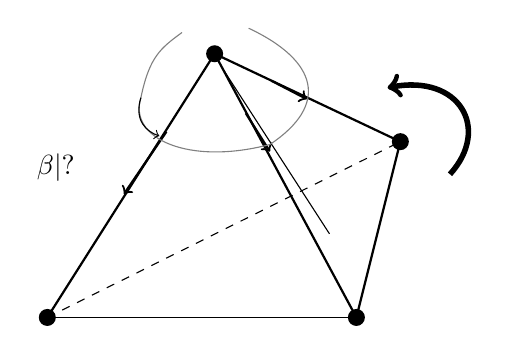
\begin{tikzpicture}[x=.018cm,y=-.018cm]
\coordinate (A) at (27,216); \coordinate (B) at (145,30);
\coordinate (C) at (245,216); \coordinate (D) at (276,92);
\draw[thick] (A)--(B)--(C)--(D)--(B);
\draw[thin] (A)--(C);
\draw[dashed] (A)--(D);
\draw[thin] (151,41)--(226,157);
\draw[->,thick] (111,85)--(81,129);
\draw[->,thick] (167,72)--(184,99);
\draw[->,thick] (185,49)--(210,62);
\foreach \p in {A,B,C,D}{\fill (\p) circle (6);}
\draw[gray] (169,12)..controls(218,35)and(226,66)..(184,94)..controls(127,109)and(84,90)..(93,61)..controls(99,32)and(107,26)..(122,15);
\draw[->] (93,61)..controls(88,77)and(97,85)..(106,88);
\draw[line width=2pt,->] (311,115)..controls(340,83)and(318,44)..(267,54);
\node at (33,110) {$\unsure{\beta|?}$};
\end{tikzpicture}}

\diagram{\begin{tikzcd}[column sep=small]
\left.\begin{array}{l}\deleted{\deleted{6}\inserted{4}\text{ hexagones}}\\\deleted{4\text{ sommets}}\end{array}\right\}
\arrow[r,bend left]
&
\begin{array}{l}
8\text{ triangles}\\
4\text{ sommets d'ordre }6\\
12\text{ arêtes}
\end{array}
\end{tikzcd}}

\[
G_{\unsure{4}}
\]

\[
\deleted{\unsure{\widetilde{\mathfrak S}_3}}:
\qquad \mu_6\times(\mathbb Z/2\mathbb Z)^2
\]
\[
\mu_4\times(\mathbb Z/2\mathbb Z)^2
\]

\uline{Hexagone}

\uline{Orienté}

\figure{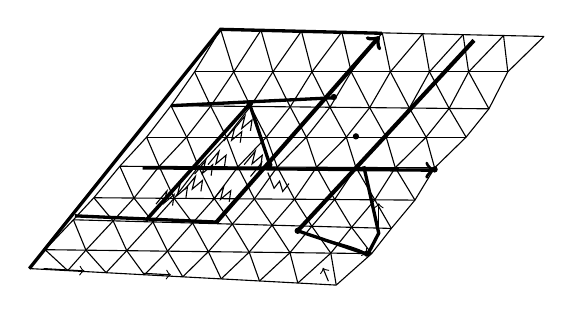
\begin{tikzpicture}[x=.010cm,y=-.010cm]
\draw (10.0,322.0)--(400.0,343.0);
\draw (30.0,298.0)--(445.0,303.0);
\draw (66.0,260.0)--(470.0,271.0);
\draw (92.0,232.0)--(500.0,235.0);
\draw (125.0,192.0)--(525.0,194.0);
\draw (159.0,155.0)--(565.0,155.0);
\draw (190.0,115.0)--(594.0,119.0);
\draw (220.0,72.0)--(618.0,72.0);
\draw (253.0,18.0)--(664.0,27.0);
\draw (10.0,322.0)--(30.0,298.0)--(66.0,260.0)--(92.0,232.0)--(125.0,192.0)--(159.0,155.0)--(190.0,115.0)--(220.0,72.0)--(253.0,18.0);
\draw (58.8,324.6)--(81.9,298.6)--(116.5,261.4)--(143.0,232.4)--(175.0,192.2)--(209.8,155.0)--(240.5,115.5)--(269.8,72.0)--(304.4,19.1);
\draw (107.5,327.2)--(133.8,299.2)--(167.0,262.8)--(194.0,232.8)--(225.0,192.5)--(260.5,155.0)--(291.0,116.0)--(319.5,72.0)--(355.8,20.2);
\draw (156.2,329.9)--(185.6,299.9)--(217.5,264.1)--(245.0,233.1)--(275.0,192.8)--(311.2,155.0)--(341.5,116.5)--(369.2,72.0)--(407.1,21.4);
\draw (205.0,332.5)--(237.5,300.5)--(268.0,265.5)--(296.0,233.5)--(325.0,193.0)--(362.0,155.0)--(392.0,117.0)--(419.0,72.0)--(458.5,22.5);
\draw (253.8,335.1)--(289.4,301.1)--(318.5,266.9)--(347.0,233.9)--(375.0,193.2)--(412.8,155.0)--(442.5,117.5)--(468.8,72.0)--(509.9,23.6);
\draw (302.5,337.8)--(341.2,301.8)--(369.0,268.2)--(398.0,234.2)--(425.0,193.5)--(463.5,155.0)--(493.0,118.0)--(518.5,72.0)--(561.2,24.8);
\draw (351.2,340.4)--(393.1,302.4)--(419.5,269.6)--(449.0,234.6)--(475.0,193.8)--(514.2,155.0)--(543.5,118.5)--(568.2,72.0)--(612.6,25.9);
\draw (400.0,343.0)--(445.0,303.0)--(470.0,271.0)--(500.0,235.0)--(525.0,194.0)--(565.0,155.0)--(594.0,119.0)--(618.0,72.0)--(664.0,27.0);
\draw (30.0,298.0)--(58.8,324.6);
\draw (81.9,298.6)--(107.5,327.2);
\draw (133.8,299.2)--(156.2,329.9);
\draw (185.6,299.9)--(205.0,332.5);
\draw (237.5,300.5)--(253.8,335.1);
\draw (289.4,301.1)--(302.5,337.8);
\draw (341.2,301.8)--(351.2,340.4);
\draw (393.1,302.4)--(400.0,343.0);
\draw (66.0,260.0)--(81.9,298.6);
\draw (116.5,261.4)--(133.8,299.2);
\draw (167.0,262.8)--(185.6,299.9);
\draw (217.5,264.1)--(237.5,300.5);
\draw (268.0,265.5)--(289.4,301.1);
\draw (318.5,266.9)--(341.2,301.8);
\draw (369.0,268.2)--(393.1,302.4);
\draw (419.5,269.6)--(445.0,303.0);
\draw (92.0,232.0)--(116.5,261.4);
\draw (143.0,232.4)--(167.0,262.8);
\draw (194.0,232.8)--(217.5,264.1);
\draw (245.0,233.1)--(268.0,265.5);
\draw (296.0,233.5)--(318.5,266.9);
\draw (347.0,233.9)--(369.0,268.2);
\draw (398.0,234.2)--(419.5,269.6);
\draw (449.0,234.6)--(470.0,271.0);
\draw (125.0,192.0)--(143.0,232.4);
\draw (175.0,192.2)--(194.0,232.8);
\draw (225.0,192.5)--(245.0,233.1);
\draw (275.0,192.8)--(296.0,233.5);
\draw (325.0,193.0)--(347.0,233.9);
\draw (375.0,193.2)--(398.0,234.2);
\draw (425.0,193.5)--(449.0,234.6);
\draw (475.0,193.8)--(500.0,235.0);
\draw (159.0,155.0)--(175.0,192.2);
\draw (209.8,155.0)--(225.0,192.5);
\draw (260.5,155.0)--(275.0,192.8);
\draw (311.2,155.0)--(325.0,193.0);
\draw (362.0,155.0)--(375.0,193.2);
\draw (412.8,155.0)--(425.0,193.5);
\draw (463.5,155.0)--(475.0,193.8);
\draw (514.2,155.0)--(525.0,194.0);
\draw (190.0,115.0)--(209.8,155.0);
\draw (240.5,115.5)--(260.5,155.0);
\draw (291.0,116.0)--(311.2,155.0);
\draw (341.5,116.5)--(362.0,155.0);
\draw (392.0,117.0)--(412.8,155.0);
\draw (442.5,117.5)--(463.5,155.0);
\draw (493.0,118.0)--(514.2,155.0);
\draw (543.5,118.5)--(565.0,155.0);
\draw (220.0,72.0)--(240.5,115.5);
\draw (269.8,72.0)--(291.0,116.0);
\draw (319.5,72.0)--(341.5,116.5);
\draw (369.2,72.0)--(392.0,117.0);
\draw (419.0,72.0)--(442.5,117.5);
\draw (468.8,72.0)--(493.0,118.0);
\draw (518.5,72.0)--(543.5,118.5);
\draw (568.2,72.0)--(594.0,119.0);
\draw (253.0,18.0)--(269.8,72.0);
\draw (304.4,19.1)--(319.5,72.0);
\draw (355.8,20.2)--(369.2,72.0);
\draw (407.1,21.4)--(419.0,72.0);
\draw (458.5,22.5)--(468.8,72.0);
\draw (509.9,23.6)--(518.5,72.0);
\draw (561.2,24.8)--(568.2,72.0);
\draw (612.6,25.9)--(618.0,72.0);
\draw[very thick] (10,322)--(253,18)--(458,23);
\draw[line width=1.3pt] (158,261)--(290,113);
\draw[line width=1.5pt,->] (247,264)--(455,27);
\draw[line width=1.5pt] (351,274)--(575,32);
\draw[very thick] (190,115)--(396,105);
\draw[very thick,->] (154,194)--(525,197);
\draw[very thick] (290,113)--(315,188);
\draw[very thick] (68,255)--(250,263);
\draw[very thick] (351,274)--(440,304)--(454,277)--(435,192);
\draw[->] (454,277)--(454,239);
\draw[->] (351,274)..controls(390,288)and(424,293)..(440,304);
\foreach \p in {(290,113),(315,190),(397,104),(425,154),(525,196),(351,274),(439,303)}{\fill \p circle (4);}
\begin{scope}\clip (151,257)--(289,116)--(315,190)--(247,260)--cycle;
\foreach \x/\y in {171/240,188/230,207/222,220/202,237/190,257/160,270/145,283/190,291/205,243/235}{\draw (\x,\y)--++(14,-17)--++(-4,16)--++(13,-11)--++(-2,14);}
\end{scope}
\draw (313,200)--(321,220)--(328,211)--(332,224)--(340,214);
\draw[->] (28,322)--(80,325); \draw[->] (155,328)--(190,330);
\draw[->] (390,338)--(383,321);
\end{tikzpicture}}

\margin{trois arêtes\\trois sommets}

\uline{Carré orienté}

\figure{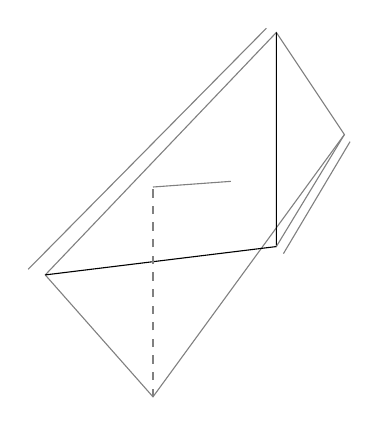
\begin{tikzpicture}[x=.018cm,y=-.018cm]
\draw[gray] (32,199)--(195,28)--(243,100)--(108,285)--cycle;
\draw (32,199)--(195,179)--(195,28);
\draw[gray] (195,179)--(243,100);
\draw[dashed,gray] (108,285)--(108,137);
\draw[gray] (108,137)--(163,133);
\draw[gray] (20,195)--(188,25);
\draw[gray] (200,184)--(247,105);
\end{tikzpicture}}

\figure{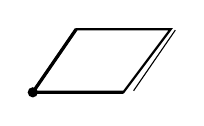
\begin{tikzpicture}[scale=1]
\draw[thick] (0,0)--(.55,.8)--(1.75,.8)--(1.15,0)--cycle;
\draw[very thick] (0,0)--(.55,.8) (0,0)--(1.15,0);
\draw[thin] (1.28,.02)--(1.81,.79);
\fill (0,0) circle (.065);
\end{tikzpicture}}

\figure{\begin{tikzpicture}[scale=.8]
\draw[->] (0,1.3)--(0,0);
\draw[gray] (.08,1.4)--(1.2,1.4)--(1.2,0);
\draw[gray] (.08,1.3)--(.3,1.04);
\draw[gray] (.05,-.03)--(.32,.04);
\end{tikzpicture}}

\figure{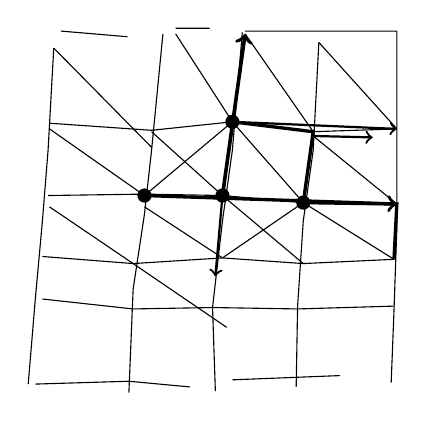
\begin{tikzpicture}[x=.018cm,y=-.018cm]
\draw (28,28)--(24,100)--(20,150)--(15,205)--(10,265);
\draw (105,18)--(97,100)--(92,145)--(84,198)--(81,271);
\draw (161,17)--(154,100)--(147,150)--(140,211)--(142,270);
\draw (215,24)--(211,100)--(204,150)--(200,210)--(199,267);
\draw (270,16)--(270,100)--(270,155)--(268,213)--(266,264);
\draw (33,16)--(80,20) (114,14)--(138,14) (163,16)--(270,16);
\draw (25,81)--(97,86)--(154,80)--(211,87)--(270,85);
\draw (24,132)--(92,131)--(147,132)--(204,137)--(270,138);
\draw (20,175)--(84,180)--(147,176)--(204,180)--(268,177);
\draw (20,205)--(84,212)--(140,211)--(200,212)--(268,210);
\draw (15,265)--(81,263)--(124,267) (154,262)--(230,259);
\draw (28,28)--(97,98) (114,18)--(154,80) (163,18)--(211,87) (215,24)--(270,85);
\draw (25,85)--(92,132) (97,87)--(147,132) (154,80)--(204,137) (211,90)--(270,138);
\draw (25,140)--(84,180)--(150,225) (92,140)--(147,176) (147,132)--(204,180) (204,137)--(268,177);
\draw[thin] (92,132)--(154,80) (147,176)--(204,137);
\draw[line width=1.3pt,->] (147,132)--(163,18);
\draw[very thick,->] (92,132)--(270,138);
\draw[very thick] (154,80)--(211,87)--(204,137)--(270,138)--(268,177);
\draw[thick,->] (147,132)--(142,189);
\draw[thick,->] (154,80)--(270,85);
\draw[thick,->] (211,90)--(253,91);
\foreach \p in {(92,132),(147,132),(154,80),(204,137)}{\fill \p circle (5);}
\end{tikzpicture}}

\figure{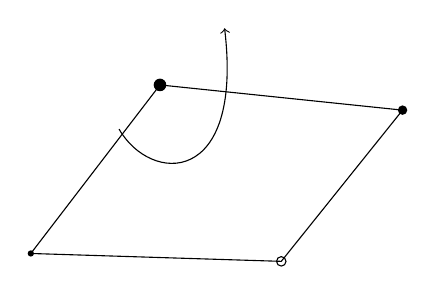
\begin{tikzpicture}[x=.020cm,y=-.020cm]
\draw (20,148)--(102,41)--(256,57)--(179,153)--cycle;
\fill (102,41) circle (4); \fill (256,57) circle (3);
\fill (20,148) circle (2);
\draw (179,153) circle (3);
\draw[->] (76,69)..controls(96,104)and(155,106)..(143,5);
\end{tikzpicture}}

$\deleted{2}\inserted{4}$ carrés

$8$ arêtes

$4$ sommets

\diagram{\fbox{\begin{tikzcd}
E_{\varepsilon,+}\arrow[r,bend left,very thick]\arrow[d,leftrightarrow,very thick]&
E_{\varepsilon,-}\arrow[l,bend left,very thick]\arrow[d,leftrightarrow,very thick]\\
\unsure{E_Q|\overline E_Q}\arrow[r,very thick]&\unsure{E_H|\overline E_H}
\end{tikzcd}}}

\margin{22}

\scanpage{24}
\margin{Mireille \& enfants}
\figure{
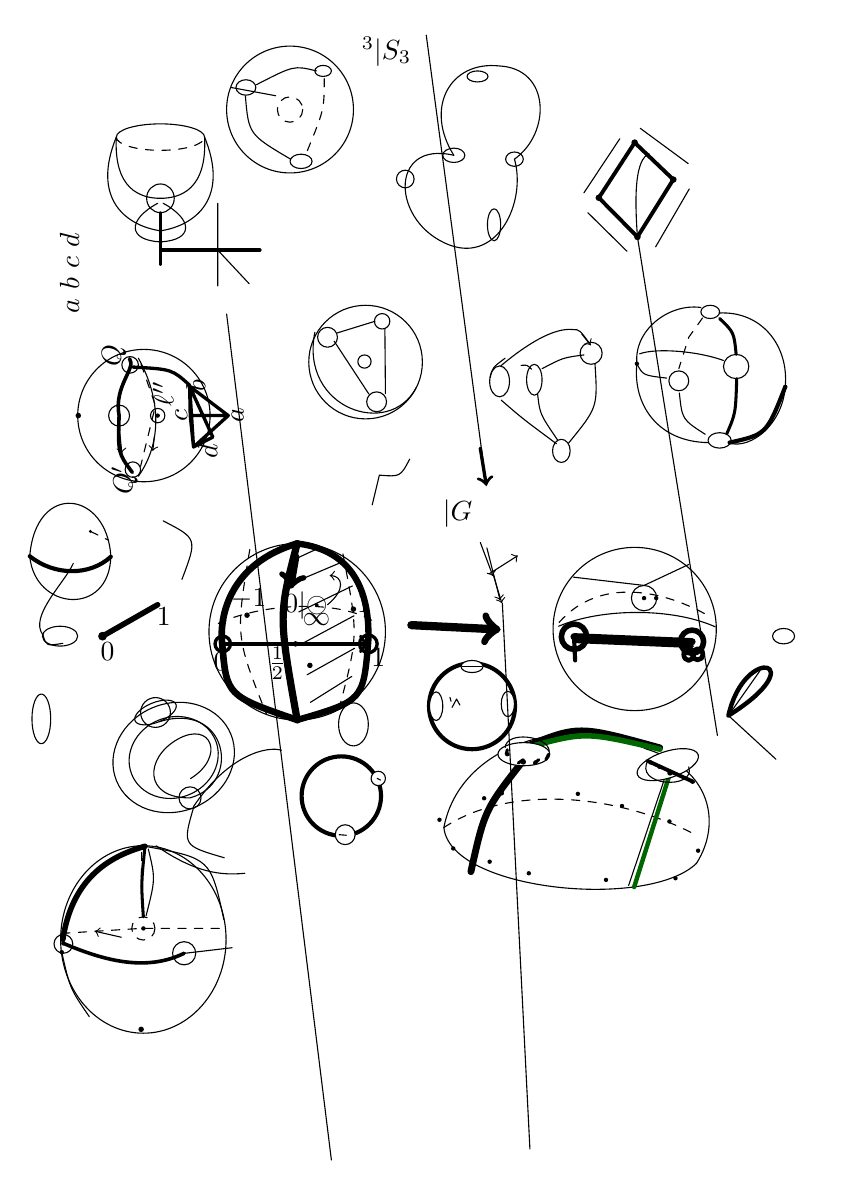
\begin{tikzpicture}[x=.007cm,y=-.007cm,line cap=round,line join=round]
\begin{scope}[shift={(330,425)}]
\draw (-80,-80) arc[start angle=180,end angle=360,x radius=80,y radius=24];
\draw[dashed] (-80,-80) arc[start angle=180,end angle=0,x radius=80,y radius=24];
\draw (-80,-80) .. controls (-125,30) and (-65,80) .. (0,90) .. controls (65,80) and (125,30) .. (80,-80);
\draw (-80,-80) .. controls (-85,15) and (-36,31) .. (0,31) .. controls (36,31) and (85,15) .. (80,-80);
\draw (0,31) ellipse (25 and 26);
\draw (-5,40) .. controls (-60,70) and (-60,107) .. (0,110) .. controls (60,107) and (60,70) .. (5,40);
\draw[line width=1.4pt] (0,58)--(0,125)--(180,125) (0,98)--(0,150);
\draw (104,40)--(104,190) (104,125)--(161,186);
\end{scope}
\begin{scope}[shift={(565,295)}]
\draw (0,0) circle (115);
\draw (-80,-40) ellipse (18 and 14) (20,94) ellipse (20 and 13) (60,-70) ellipse (15 and 10);
\draw (-81,-25) .. controls (-75,45) .. (1,90);
\draw (-61,-45) .. controls (7,-80) .. (48,-70);
\draw[dashed] (62,-56) .. controls (62,0) .. (30,78) (0,0) circle (23);
\draw (-107,-40)--(-26,-25);
\end{scope}
\node at (740,190) {\(\unsure{\circlearrowleft^{3}|\mathfrak S_3}\)};
\begin{scope}[shift={(900,380)}]
\draw (-38,-2) .. controls (-92,-88) and (-45,-174) .. (45,-164) .. controls (137,-159) and (139,-43) .. (72,5);
\draw (-38,-2) ellipse (20 and 13) (72,5) ellipse (16 and 13) (5,-145) ellipse (19 and 10);
\draw (-38,-2) .. controls (-157,-30) and (-152,121) .. (-45,161) .. controls (42,193) and (94,82) .. (72,5);
\draw (-126,41) circle (16);
\draw (35,124) ellipse (12 and 29);
\end{scope}
\draw (812,160)--(921,977);
\draw[->,line width=1.2pt] (910,909)--(921,977);
\node at (869,1028) {\(\unsure{\circlearrowleft|G}\)};
\draw[->] (910,1080)--(933,1141);
\draw[->] (926,1137)--(978,1104);
\draw[->] (922,1090)--(946,1185);
\draw[->] (934,1140)--(949,1190);
\draw (450,666)--(640,2200);
\draw (714,1012)--(727,958) .. controls (765,961) .. (782,929);
\draw (335,1041) .. controls (397,1073) .. (369,1147);
\begin{scope}[shift={(1190,440)}]
\draw[line width=1.4pt] (0,-85)--(-65,15)--(5,86)--(70,-18)--cycle;
\draw (5,86) .. controls (-1,4) and (2,-54) .. (26,-65);
\foreach \x/\y in {0/-85,-65/15,5/86,70/-18}{\fill (\x,\y) circle (6);}
\draw (-92,6)--(-27,-92) (-85,42)--(-14,112) (38,104)--(99,-1) (10,-111)--(97,-47);
\end{scope}
\draw (1195,526)--(1340,1430);
\begin{scope}[shift={(300,850)},rotate=-90]
\draw (0,0) circle (120);
\draw[line width=1.3pt] (-103,26) .. controls (-86,13) and (-54,55) .. (0,45) .. controls (68,47) .. (103,21);
\draw (-104,10) .. controls (-34,-29) and (46,-35) .. (110,10);
\draw[dashed] (-93,5)--(-18,-21)--(92,6);
\draw (-92,25) circle (15) (98,20) circle (14) (0,-25) circle (13);
\draw (0,45) circle (19);
\fill (0,-25) circle (4);
\fill (0,119) circle (5);
\draw[line width=1.2pt] (-88,20) .. controls (-84,-51) .. (-55,-83);
\draw[line width=1.2pt] (-53,-83)--(0,-153)--(57,-90)--(-53,-83)--(0,-84)--(0,-153) (-53,-83)--(39,-125)--(57,-90) (0,-84)--(57,-90);
\node[rotate=90] at (0,-170) {\(a\)};
\node[rotate=90] at (-55,-94) {\(\unsure{b}\)};
\node[rotate=90] at (0,-68) {\(\unsure{c}\)};
\node[rotate=90] at (64,-116) {\(d\)};
\node[rotate=90] at (40,-75) {\(\circlearrowleft\)};
\node[rotate=90] at (-40,-35) {\(\ell''\)};
\node[rotate=90] at (-108,54) {\(Q\)};
\node[rotate=90] at (117,35) {\(Q'\)};
\draw[->] (18,45)--(68,40);
\draw[->] (38,-19) .. controls (51,-18) .. (64,-16);
\end{scope}
\node[rotate=90] at (165,592) {\(a\ b\ c\ d\)};
\begin{scope}[shift={(702,753)}]
\draw (0,0) circle (103);
\draw (-69,-45) circle (18) (30,-74) circle (14) (20,72) circle (18) (-2,-1) circle (12);
\draw (-57,-38)--(6,58) (36,57)--(35,-60) (17,-74)--(-51,-53);
\draw (-92,-54) .. controls (-120,84) and (43,140) .. (92,46);
\end{scope}
% Middle sphere: the short stroke left of the central oval remains free.
\begin{scope}
\draw (947,760) .. controls (991,723) and (1042,690) .. (1078,694) .. controls (1090,694) .. (1110,722);
\draw[->] (1094,702)--(1110,722);
\draw (928,781) .. controls (932,763) .. (955,746);
\draw (948,822) .. controls (986,855) .. (1048,901);
\draw (1118,756) .. controls (1123,835) .. (1070,900);
\draw (945,788) ellipse (18 and 28) (1111,737) circle (20) (1057,914) ellipse (16 and 21) (1008,785) ellipse (14 and 28);
\draw (1022,765) .. controls (1060,745) .. (1098,740);
\draw (1014,811) .. controls (1018,847) .. (1050,894);
\draw (984,759) .. controls (995,758) .. (1003,766);
\end{scope}
% Right sphere: four holes, with two additional filled boundary points.
\begin{scope}
\draw (1194,756) .. controls (1188,695) and (1252,646) .. (1310,654);
\draw (1343,664) .. controls (1419,660) and (1470,722) .. (1463,798) .. controls (1458,866) and (1401,911) .. (1362,900);
\draw (1324,899) .. controls (1231,898) and (1186,829) .. (1194,756);
\draw (1327,662) ellipse (17 and 12) (1270,787) circle (18) (1374,761) ellipse (23 and 22) (1344,895) ellipse (21 and 14);
\draw[line width=1.1pt] (1344,674) .. controls (1370,699) .. (1374,739) (1375,783) .. controls (1373,846) .. (1357,883);
\draw[line width=1.5pt] (1362,899) .. controls (1429,884) .. (1463,798);
\draw[dashed] (1313,673)--(1288,708)--(1270,765);
\draw (1271,809) .. controls (1276,857) .. (1318,884);
\draw (1199,738) .. controls (1229,727) and (1304,733) .. (1351,750);
\draw (1194,756) .. controls (1205,777) .. (1248,782);
\fill (1194,756) circle (4) (1463,798) circle (4);
\end{scope}
\begin{scope}[shift={(168,1110)}]
\draw (-75,-5) .. controls (-64,-142) and (66,-124) .. (72,-4) .. controls (69,105) and (-66,94) .. (-75,-5);
\draw[line width=1.5pt] (-75,-5) .. controls (-30,31) and (34,31) .. (72,-4);
\fill (35,-50) circle (3);
\draw[dashed] (35,-50)--(68,-34);
\draw (4,8) .. controls (-12,44) and (-77,104) .. (-51,138) .. controls (-45,158) .. (-15,153);
\draw (-20,140) ellipse (32 and 18);
\end{scope}
\draw[line width=2pt] (225,1250)--(325,1193);
\fill (225,1250) circle (8);
\node at (234,1278) {\(0\)};
\node at (336,1214) {\(1\)};
\draw (114,1400) ellipse (17 and 45);
\begin{scope}[shift={(578,1242)}]
\draw (0,0) circle (160);
\draw[line width=2.4pt] (0,-160) .. controls (-121,-125) and (-142,-29) .. (-136,22) .. controls (-128,116) .. (0,160);
\draw[line width=2.3pt] (0,-160) .. controls (102,-148) and (132,-71) .. (129,16) .. controls (120,125) .. (0,160);
\draw[line width=2.6pt] (0,-160) .. controls (-34,-30) .. (0,160);
\draw[->,line width=2.4pt] (-2,-136)--(-12,-78);
\draw[->,line width=1.4pt] (-138,22)--(131,22);
\draw[dashed] (-143,-15) .. controls (-71,-49) and (72,-63) .. (143,-16);
\draw[dashed] (-86,-149) .. controls (-112,8) .. (-56,149) (83,-141) .. controls (111,6) .. (76,139);
\foreach \x/\y in {-135/22,-3/22,129/22,-91/-30,102/-41,23/61,0/156}{\fill (\x,\y) circle (5);}
\draw[line width=1.2pt] (-135,22) circle (14) (129,22) circle (16);
\foreach \a/\b/\c/\d in {3/-135/42/-153,0/-92/78/-125,3/-36/100/-83,8/22/103/-29,18/78/104/30,24/128/99/81}{\draw (\a,\b)--(\c,\d);}
\draw[->] (55,-49) .. controls (89,-77) and (82,-101) .. (59,-102);
\node at (-88,-60) {\(-1\)};
\node at (-36,57) {\(\frac12\)};
\node at (16,-48) {\(\unsure{0|\odot}\)};
\node at (35,-22) {\(\infty\)};
\node at (-139,55) {\(0\)};
\node at (147,46) {\(1\)};
\node at (121,-51) {\(1\)};
\end{scope}
\draw[->,line width=3pt] (785,1230)--(947,1238);
\begin{scope}[shift={(1190,1237)}]
\draw (0,0) circle (148);
\draw (-138,-5) .. controls (-57,-39) and (70,-38) .. (146,-4);
\draw[dashed] (-137,-12) .. controls (-64,-95) and (52,-72) .. (139,-21);
\draw[line width=1.4pt] (-110,22)--(104,31);
\draw[line width=2.6pt] (-110,14)--(104,23);
\draw[line width=2pt] (-110,14) circle (23) (104,23) circle (21);
\draw (17,-56) circle (23);
\draw (-111,-94)--(17,-79)--(98,-117);
\draw[line width=1.5pt] (-110,14)--(-108,57);
\draw[line width=1.7pt] (98,46) ellipse (9 and 11) (114,46) ellipse (10 and 10);
\foreach \x/\y in {-110/14,104/23,17/-56,-88/14,83/23,39/-56}{\fill (\x,\y) circle (4);}
\end{scope}
\draw (1460,1250) ellipse (20 and 14);
\draw[line width=1.6pt] (1360,1394) .. controls (1390,1261) and (1517,1296) .. (1360,1394);
\draw (1360,1394)--(1446,1473) (1360,1394)--(1417,1313);
\draw (680,1410) ellipse (27 and 39);
\begin{scope}[shift={(895,1377)}]
\draw[line width=1.5pt] (0,0) circle (78);
\draw[fill=white] (-65,0) ellipse (12 and 26) (65,-4) ellipse (12 and 23) (0,-72) ellipse (20 and 11);
\draw (-18,-72)--(18,-72);
\draw (-40,-16)--(-38,-9) (-36,2)--(-28,-13)--(-22,-2);
\end{scope}
\begin{scope}[shift={(354,1470)},rotate=22]
\draw (0,0) ellipse (112 and 98);
\draw (0,0) ellipse (82 and 73);
\draw (0,-88) ellipse (40 and 18);
\draw (0,-88) circle (27);
\draw (0,79) circle (20);
\draw (0,-70) .. controls (130,-59) and (97,91) .. (0,79) .. controls (-79,48) and (-49,-19) .. (19,-28) .. controls (89,-37) and (88,34) .. (14,47);
\draw (0,97) .. controls (-45,154) .. (17,203);
\draw (0,96) .. controls (96,31) and (167,45) .. (186,61);
\end{scope}
\begin{scope}[shift={(658,1540)}]
\draw[line width=1.5pt] (0,0) circle (72);
\draw[fill=white] (7,70) circle (18) (67,-32) circle (13);
\draw[dashed] (-66,-32)--(-44,-59);
\draw (-4,70)--(9,71) (65,-32)--(71,-29);
\end{scope}
\begin{scope}[shift={(299,1800)}]
\draw (0,0) ellipse (150 and 170);
\draw[line width=2pt] (-146,0) .. controls (-130,-105) and (-69,-149) .. (3,-169);
\draw (3,-169) .. controls (122,-147) .. (146,-36);
\draw[line width=1.3pt] (-145,7) .. controls (-68,40) and (7,58) .. (74,25);
\draw (76,25)--(161,15);
\draw[dashed] (-148,-11)--(-5,-20)--(139,-20);
\draw (-145,8) circle (17) (74,25) circle (21);
\draw[dashed] (0,-20) circle (21);
\draw[line width=1.1pt] (3,-169) .. controls (-4,-102) .. (0,-41);
\draw (9,-164) .. controls (22,-110) .. (5,-43);
\draw[dashed] (-3,-158)--(-4,-95);
\fill (0,-20) circle (4) (-145,7) circle (4) (-148,23) circle (4);
\draw[->] (-40,-4)--(-88,-15);
\draw (23,-170) .. controls (95,-120) and (142,-116) .. (184,-120);
\draw (-148,23) .. controls (-133,89) .. (-98,140);
\fill (-4,163) circle (5);
\end{scope}
\begin{scope}[shift={(1080,1557)}]
\draw (-236,40) .. controls (-208,-108) and (-15,-171) .. (132,-102) .. controls (249,-66) and (268,33) .. (222,105);
\draw (-236,40) .. controls (-225,155) and (134,190) .. (222,105);
\draw[dashed] (-236,40) .. controls (-115,-40) and (83,-20) .. (222,54);
\draw[line width=2.5pt] (-187,120) .. controls (-162,8) .. (-91,-83);
\draw[line width=2.2pt] (-91,-106) .. controls (8,-146) .. (156,-105);
\draw[green!40!black,line width=2pt] (-89,-104) .. controls (20,-134) .. (156,-102);
\draw[green!40!black,line width=1.6pt] (174,-58)--(109,148);
\draw (164,-48)--(99,145);
\draw[fill=white] (-91,-93) ellipse (47 and 21);
\draw (-125,-105) .. controls (-122,-136) and (-47,-126) .. (-45,-99);
\draw[fill=white,rotate around={18:(170,-74)}] (170,-74) ellipse (58 and 24);
\draw (135,-83) .. controls (105,-35) and (222,-27) .. (208,-70);
\draw[line width=1.1pt] (-123,-93)--(-121,-101) (-101,-77)--(-92,-83) (-72,-76)--(-64,-83) (-51,-83)--(-46,-93);
\fill (-121,-93) circle (4) (-92,-79) circle (5) (-70,-78) circle (4);
\draw[line width=1.4pt] (133,-81)--(216,-43);
\fill (139,-78) circle (4) (155,-70) circle (4) (174,-59) circle (5) (215,-43) circle (4);
\foreach \x/\y in {-244/26,-219/78,-153/102,-82/123,58/135,184/132,225/82,-163/-13,-131/-22,7/-21,87/1,173/29}{\fill (\x,\y) circle (4);}
\end{scope}
\draw (950,1190)--(1000,2180);
\end{tikzpicture}
}% crop-candidate: scan 24
\margin{\(\operatorname{diag}_Q\simeq\omega_Q\)\quad
\(\operatorname{diag}_Q\wedge\omega_Q\simeq\operatorname{codiag}_Q\)}
\margin{\unsure{avec} un ens à trois éléments, on fait \(3\times2=6\) cartes elliptiques de type \((1,1)\)}
avec un ens \(I\) de card \(4\),
on peut trouver \(\unsure{17|14}\) \unsure{cartes|points|ponts} \unsure{on|ou|or} canoniques \inserted{de type \((0,4)\)}
\((14=3\times4+\deleted{3\times}2)\)
dont deux tétraédrales,
\deleted{\unsure{quatre}}\inserted{trois} carrés, \deleted{deux} \(2\times3=6\)
assemblages de \deleted{\unsure{F}} ``\(J\)'' droits,
\(6=2\times3\) assemblages de \inserted{\(1\)} \(J\) gauches.
\margin{23}

\scanpage{25}

\figure{\begin{tikzpicture}[x=.009cm,y=-.009cm,line cap=round,
 every node/.style={inner sep=0pt,anchor=west,font=\small}]
% One table: the descriptors and the mathematical labels share their manuscript rows.
\node[anchor=center,font=\Large] at (264,65) {$A$};
\node at (320,72) {triangle};
\node[anchor=center,font=\Large] at (246,143) {$\vec T$};
\node at (306,153) {tétraèdre orienté};
\node[anchor=center,font=\Large] at (246,229) {$\overset{\deleted{\rightarrow}}{Q}$};
\node at (304,238) {carré};
\node at (419,236) {\deleted{orienté}};
\node[anchor=center,font=\Large] at (253,305) {$\unsure{\bar Q}$};
\node at (320,311) {\deleted{hexagone}};
\node at (514,306) {carré orienté};
\node[anchor=center,font=\Large] at (262,376) {$\bar H$};
\node at (382,389) {hexagone orienté};

\node[font=\Large] at (883,67) {$\Sigma_A$};
\node[anchor=north west,font=\Large] at (880,111) {
  \begin{tikzcd}[row sep=5pt,column sep=0pt]
  \Sigma_T \arrow[d,leftrightarrow,bend left=45,start anchor=east,end anchor=east]\\
  \Sigma_Q
  \end{tikzcd}};
\node[font=\Large] at (905,300) {$E_{\vec Q}$};
\node[font=\Large] at (908,376) {$E_{\vec H}$};
\node[font=\Large] at (1107,78) {$(0,3)$};
\node[font=\Large] at (1097,158) {$(0,4)$};
\node[font=\Large] at (1106,302) {$(1,1)$};
\node[font=\Large] at (1086,485) {$(0,5)$};
\node[font=\Large] at (1085,588) {$(1,2)$};
% Closing brace over Sigma_Q, E_{vec Q}, E_{vec H}.
\draw[line width=.45pt] (1086,220)
 .. controls (1106,211) and (1100,237) .. (1094,265)
 .. controls (1087,294) and (1095,306) .. (1110,309)
 .. controls (1094,311) and (1091,325) .. (1095,352)
 .. controls (1101,380) and (1098,400) .. (1086,406);
% Separator and closing dimension braces, with the labels to their right.
\draw[line width=.4pt] (1340,41) -- (1335,637);
\node[font=\Large] at (1371,77) {$d=0$};
\node[font=\Large] at (1375,154) {$d=1$};
\draw[line width=.45pt] (1354,145)
 .. controls (1365,150) and (1360,185) .. (1356,222)
 .. controls (1351,264) and (1357,282) .. (1377,286)
 .. controls (1357,289) and (1356,315) .. (1359,354)
 .. controls (1364,392) and (1364,408) .. (1352,411);
\draw[line width=.45pt] (1354,467)
 .. controls (1368,462) and (1357,489) .. (1354,511)
 .. controls (1351,531) and (1359,540) .. (1372,539)
 .. controls (1356,543) and (1357,564) .. (1361,585)
 .. controls (1367,607) and (1361,617) .. (1353,619);
\node[font=\Large] at (1392,530) {$d=2$};

% Two blank name slots, aligned with the last two ordered pairs.
\draw[line width=.3pt] (291,535) .. controls (304,530) and (316,530) .. (327,534);
\draw[line width=.3pt] (360,531) .. controls (375,525) and (389,529) .. (401,530);
\draw[line width=.3pt] (424,527) .. controls (450,521) and (477,517) .. (496,524);
\draw[line width=.3pt] (527,522) .. controls (547,511) and (570,516) .. (589,516);
\draw[line width=.3pt] (607,519) .. controls (654,509) and (697,504) .. (719,501)
 .. controls (733,501) and (744,503) .. (754,503);
\draw[line width=.3pt] (307,645) .. controls (323,638) and (341,640) .. (354,644);
\draw[line width=.3pt] (370,644) .. controls (390,637) and (404,647) .. (425,642)
 .. controls (451,630) and (466,643) .. (497,635)
 .. controls (535,623) and (557,631) .. (588,626)
 .. controls (624,615) and (646,619) .. (679,612)
 -- (808,598);
\draw[line width=.35pt] (726,875) .. controls (736,874) and (743,876) .. (751,878);

% Quadrilateral with four marked vertices and four unlabelled exterior edges.
\draw[line width=.7pt] (993,881) -- (1073,683) -- (1197,780) -- (1126,962) -- cycle;
\draw[line width=.7pt] (1073,683) -- (1046,552);
\draw[line width=.7pt] (1197,780) -- (1344,717);
\draw[line width=.7pt] (993,881) -- (854,929);
\draw[line width=.7pt] (1126,962) .. controls (1139,985) and (1142,1034) .. (1163,1101);
\foreach \x/\y in {993/881,1073/683,1197/780,1126/962}
 {\fill (\x,\y) circle (2pt);}
\end{tikzpicture}}

\margin{24}

\scanpage{26}
\diagram{\begin{tikzcd}[column sep=large]
\begin{gathered}\text{Carte cellulaire (pas orientée) }\text{conn}\\
\text{dont tous les sommets sont}\\
\text{d'ordre }3\ \inserted{\text{ou }1}
\end{gathered}
\arrow[r,leftarrow,shift left=.6ex]\arrow[r,shift right=.6ex] & \text{cartes }\uline{\text{cellulaires}}
\end{tikzcd}}
\inserted{\(\mathrm{or}^{t}\)}\,/\,triangulée \(\simeq\)
\margin{\unsure{\(\deleted{\mathbf Z}n-\)|\(\deleted{\mathbf Z/n}\)}}
\unsure{revêtements|\deleted{revêtements}} de \(\mathbb P^1_{\mathbb C}\) ramifiés \unsure{seulement} en \(0,1,\infty\),
\figure{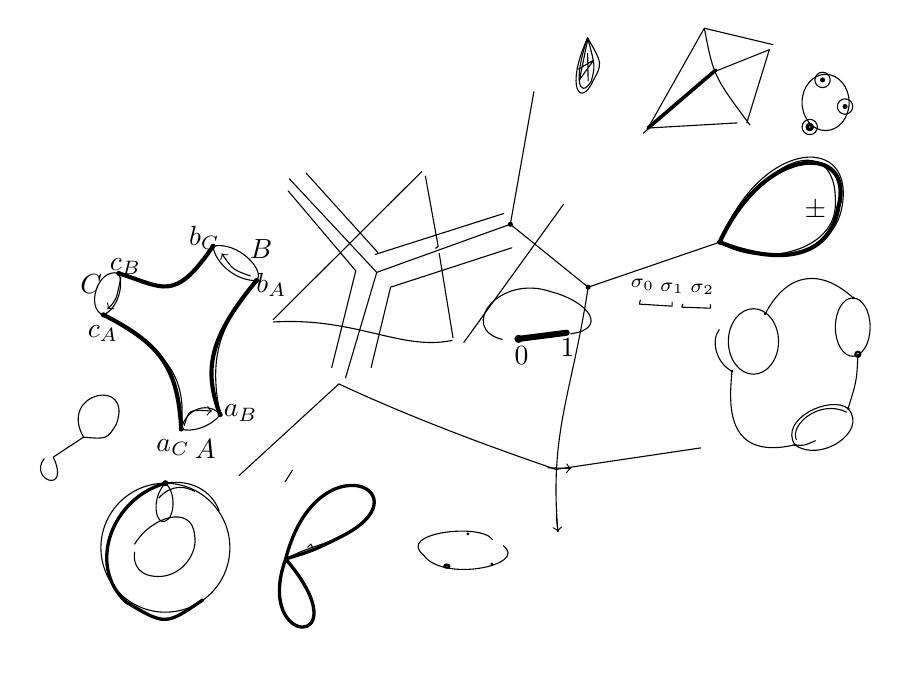
\begin{tikzpicture}[x=.0065cm,y=-.0065cm,line cap=round,line join=round]
\begin{scope}[shift={(1112,150)}]
\draw (0,-55) .. controls (-45,43) and (-13,83) .. (11,28) .. controls (29,-5) .. (0,-55);
\draw (0,-55) .. controls (-28,24) and (-17,67) .. (7,30) .. controls (15,0) .. (0,-55);
\draw (0,-51)--(-16,27)--(12,-12)--(-18,6) (0,-25)--(1,29);
\end{scope}
\begin{scope}[shift={(1340,170)}]
\draw (-110,101)--(0,-94)--(134,-62) (127,-52)--(83,91) (0,-94)..controls (18,-1)..(89,95) (-110,101)--(64,91);
\draw[line width=1.3pt] (-110,101)--(22,-12);
\draw (-119,111)--(17,-8)--(127,-52);
\end{scope}
\begin{scope}[shift={(1577,221)}]
\draw (0,0) ellipse (46 and 55);
\foreach \x/\y in {-6/-44,38/8,-31/48}{\draw (\x,\y) circle (15);}
\foreach \x/\y in {-6/-44,38/8}{\fill (\x,\y) circle (5);}
\draw[line width=1.2pt] (-31,48) circle (5);
\end{scope}
\begin{scope}[shift={(300,680)}]
\draw[line width=1.5pt] (-104,-125) .. controls (-17,-98) and (4,-67) .. (80,-178);
\draw[line width=1.5pt] (165,-111) .. controls (74,-1) and (60,62) .. (94,151);
\draw[line width=1.5pt] (-134,-44) .. controls (-17,15) and (11,64) .. (18,179);
\draw (-139,-45) .. controls (-9,26) and (29,74) .. (18,179);
\draw (165,-111) .. controls (99,-28) and (69,29) .. (94,151);
\draw (-104,-125) .. controls (-147,-137) and (-169,-54) .. (-134,-44) .. controls (-106,-56) and (-94,-101) .. (-104,-125);
\draw (80,-178) .. controls (128,-189) and (184,-130) .. (165,-111) .. controls (124,-110) and (84,-146) .. (80,-178);
\draw (18,179) .. controls (28,136) and (74,126) .. (94,151) .. controls (74,177) and (34,186) .. (18,179);
\draw[->] (153,-120) .. controls (119,-132) .. (97,-164);
\draw[->] (-100,-117) .. controls (-109,-73) .. (-126,-55);
\draw[->] (24,172) .. controls (33,141) .. (78,144);
\foreach \x/\y in {-104/-125,-134/-44,80/-178,165/-111,18/179,94/151}{\fill (\x,\y) circle (5);}
\node at (-158,-105) {\(C\)};
\node at (174,-172) {\(B\)};
\node at (65,218) {\(A\)};
\node at (-91,-138) {\(c_B\)};
\node at (-135,-8) {\(c_A\)};
\node at (63,-195) {\(b_C\)};
\node at (194,-103) {\(b_A\)};
\node at (134,148) {\(a_B\)};
\node at (2,216) {\(a_C\)};
\node at (50,-47) {\(\circlearrowleft\)};
\end{scope}
\draw (529,370)--(700,553)--(639,759) (562,359)--(702,514) (527,394)--(659,550)--(612,739);
\draw (689,739)--(727,582)--(964,505) (700,553)--(961,459) (697,518)--(948,438);
\draw (498,645)--(788,356);
\draw (795,365)--(820,502)--(815,506);
\draw (822,516)--(849,681);
\draw (498,650) .. controls (658,640) and (748,707) .. (847,686);
\draw (870,690)--(1065,420);
\draw (1007,200)--(961,459)--(1113,582)--(1370,494);
\draw (1113,582) .. controls (1081,793) and (1037,863) .. (1054,1060);
\draw (431,950)--(626,771) .. controls (780,843) and (945,902) .. (1050,938)--(1333,896);
\draw[->] (1034,935)--(1080,936);
\draw[->] (1051,1030)--(1054,1060);
\foreach \x/\y in {961/459,1113/582,1370/494}{\fill (\x,\y) circle (5);}
\begin{scope}[shift={(1370,494)}]
\draw[line width=1.5pt] (0,0) .. controls (91,-197) and (266,-191) .. (232,-69) .. controls (216,33) and (115,46) .. (0,0);
\draw (0,0) .. controls (103,-191) and (229,-203) .. (226,-79) .. controls (231,19) and (78,52) .. (0,0);
\draw (0,0) .. controls (79,-198) and (253,-210) .. (241,-84) .. controls (232,40) and (78,42) .. (0,0);
\node at (187,-61) {\(\pm\)};
\end{scope}
\node[font=\scriptsize] at (1219,578) {\(\sigma_0\)};
\node[font=\scriptsize] at (1277,584) {\(\sigma_1\)};
\node[font=\scriptsize] at (1336,586) {\(\sigma_2\)};
\draw (1215,607)--(1213,615)--(1277,619)--(1277,611) (1298,615)--(1296,621)--(1352,623)--(1352,616);
\draw (945,684) .. controls (858,662) and (938,555) .. (1041,591) .. controls (1114,610) and (1153,663) .. (1079,673);
\draw[line width=2.2pt] (977,683)--(1071,671);
\fill (977,683) circle (8);
\node at (983,715) {\(0\)};
\node at (1073,700) {\(1\)};
\begin{scope}[shift={(1510,739)}]
\draw (-51,-105) .. controls (-6,-190) and (60,-192) .. (121,-136);
\draw (130,-26) .. controls (128,25) .. (111,80);
\draw (7,151) .. controls (-139,185) and (-119,53) .. (-116,7);
\draw (-74,-51) ellipse (49 and 64);
\draw (120,-79) ellipse (34 and 57);
\draw (111,80) .. controls (76,53) and (-25,101) .. (7,151) .. controls (55,187) and (151,126) .. (111,80);
\draw (-141,-74) .. controls (-158,-52) and (-146,-8) .. (-116,7);
\draw (108,87) .. controls (54,61) and (-4,113) .. (10,141);
\draw (7,151) .. controls (24,153) .. (47,143);
\foreach \x/\y in {-51/-105,-116/7,121/-136,111/80,7/151}{\fill (\x,\y) circle (3);}
\draw[line width=.8pt] (130,-26) circle (5);
\end{scope}
\draw (127,875) .. controls (77,786) and (226,757) .. (191,850) .. controls (173,879) .. (127,875)--(68,914) .. controls (102,988) and (19,959) .. (50,917);
\begin{scope}[shift={(287,1091)}]
\draw (0,0) ellipse (126 and 126);
\draw (-60,-7) .. controls (-28,-61) and (52,-85) .. (57,-25) .. controls (64,9) and (35,52) .. (-7,56) .. controls (-52,59) and (-64,32) .. (-60,9);
\draw[line width=1.2pt] (0,-126) .. controls (-105,-97) and (-154,35) .. (-77,106) .. controls (0,152) .. (73,102);
\draw (0,-126) .. controls (-23,-102) and (-22,-64) .. (-10,-53) .. controls (15,-40) and (26,-104) .. (0,-126);
\draw (-13,-97) .. controls (12,-125) and (40,-120) .. (57,-110);
\draw (0,-126) .. controls (52,-135) and (92,-109) .. (105,-72);
\fill (0,-126) circle (6);
\end{scope}
\begin{scope}[shift={(522,1113)}]
\draw[line width=1.2pt] (0,0) .. controls (61,-237) and (282,-129) .. (107,-43) .. controls (55,-17) .. (0,0) .. controls (-64,177) and (152,178) .. (0,0);
\draw (0,0) .. controls (37,-20) and (63,-25) .. (90,-36);
\draw (43,-23)--(49,-29)--(53,-22);
\end{scope}
\draw (791,1105) .. controls (738,1062) and (903,1042) .. (926,1075);
\draw (947,1087) .. controls (998,1125) and (829,1160) .. (791,1105);
\foreach \x/\y in {878/1064,925/1123}{\fill (\x,\y) circle (3);}
\draw[line width=.8pt] (837,1127) ellipse (5 and 3);
\draw (521,962)--(535,940);
\end{tikzpicture}}% crop-candidate: scan 26
\deleted{\unsure{variétés} algébriques d}
\[
\sigma_0^2=\sigma_1^2=\sigma_2^2=(\sigma_0\sigma_2)^2=(\sigma_0\sigma_1)^3=1
\]
\(\mathbb R\)-courbes algébriques
\margin{\(\sigma_0,\sigma_1,\sigma_2\)\quad ss pts fixes}
\margin{25}

\scanpage{27}
\figure{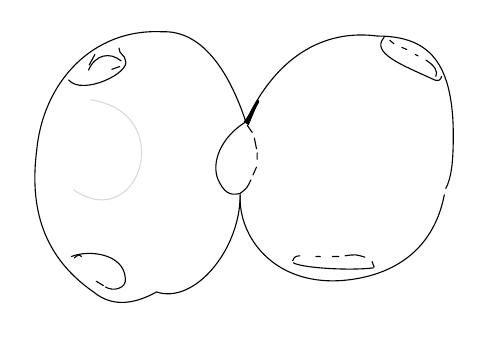
\begin{tikzpicture}[x=.009cm,y=-.009cm,line cap=round]
\draw (437,240) .. controls (407,150) and (365,111) .. (319,113)
 .. controls (220,108) and (151,185) .. (142,280)
 .. controls (130,373) and (159,436) .. (222,480)
 .. controls (251,504) and (284,495) .. (311,480)
 .. controls (364,498) and (429,421) .. (429,343);
\draw (437,240) .. controls (483,140) and (555,110) .. (622,119)
 .. controls (699,119) and (735,159) .. (729,286)
 .. controls (728,309) and (724,325) .. (719,334);
\draw (717,343) .. controls (701,425) and (640,459) .. (571,464)
 .. controls (475,470) and (426,401) .. (429,343);
\draw (437,240) .. controls (400,263) and (388,299) .. (398,322)
 .. controls (406,339) and (414,345) .. (429,341);
\draw (439,245)--(446,255) (449,263)--(452,278)
 (453,284)--(453,293) (452,304)--(447,315);
\draw (444,322) .. controls (439,333) .. (429,341);
\draw[line width=1.1pt] (454,211)--(438,240);
\fill (434,240)--(441,245)--(455,211)--cycle;
\draw (187,181) .. controls (207,204) and (276,170) .. (267,153)
 .. controls (267,146) and (258,145) .. (258,136);
\draw (215,167) .. controls (225,145) and (245,141) .. (261,154);
\draw (248,166)--(259,162) (216,160)--(224,145);
\draw (191,430) .. controls (216,420) and (265,426) .. (267,461)
 .. controls (269,475) and (250,480) .. (239,473);
\draw (195,432)..controls (201,427)..(205,430) (226,465)--(236,471);
\draw (632,121) .. controls (612,143) and (660,161) .. (699,179)
 .. controls (710,185) and (712,180) .. (713,176);
\draw (640,125)--(646,130) (657,135)--(664,138)
 (676,145)--(680,147);
\draw (691,153) .. controls (704,161) and (708,169) .. (705,176);
\draw (504,439) .. controls (519,447) and (589,450) .. (617,446);
\draw (503,436) .. controls (506,430) .. (513,429);
\draw (536,430)--(542,430) (559,430)--(568,430)
 (577,429) .. controls (592,427) .. (605,431) (615,437)--(618,445);
\draw[gray!30] (218,209) .. controls (342,227) and (287,400) .. (194,336);
\end{tikzpicture}}
\diagram{\begin{tikzcd}[column sep=large]
\left.\begin{array}{l}
4\text{ hexagones}\\16\text{ arêtes}\\10\text{ sommets}
\end{array}\right\}
\arrow[r,Rightarrow] &
\begin{array}{l}8\text{ hexagones}\\82\text{ arêtes}\\16\text{ sommets}\end{array}
\\
\begin{array}{l}(\text{dont }4\text{ ramifiés})\\\text{d'ordre}\end{array}&
\end{tikzcd}}
\begin{gather*}
2\text{ hexag.}\\9\text{ arêtes}\\6\text{ sommets}
\end{gather*}
\figure{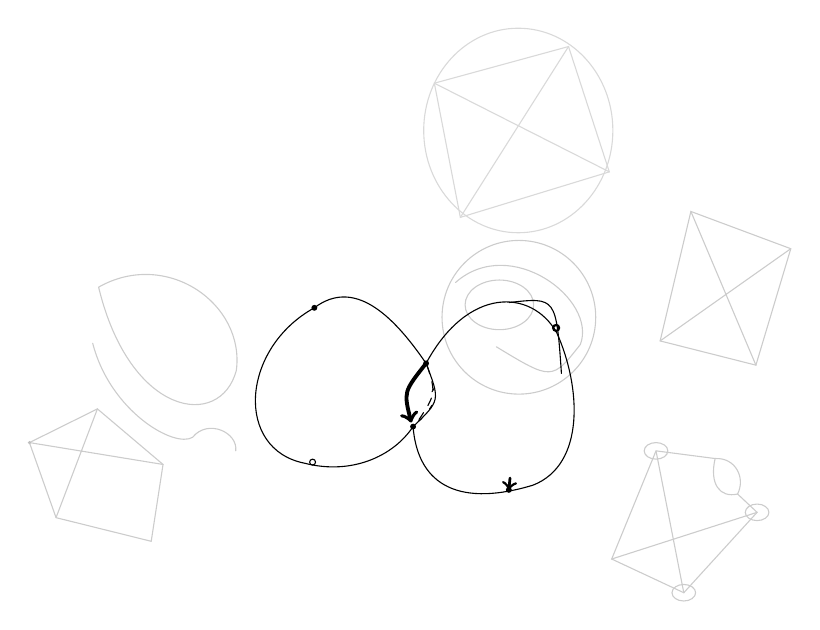
\begin{tikzpicture}[x=.0075cm,y=-.0075cm,line cap=round]
\draw[gray!30] (320,-440) ellipse (160 and 173);
\draw[gray!30] (178,-520)--(405,-582)--(474,-370)--(222,-293)--cycle;
\draw[gray!30] (178,-520)--(474,-370) (405,-582)--(222,-293);
\draw[gray!40] (-390,-175) .. controls (-275,-240) and (-142,-147) .. (-157,-34) .. controls (-184,67) and (-337,45) .. (-390,-175);
\draw[gray!40] (-400,-80) .. controls (-370,36) and (-261,98) .. (-231,79) .. controls (-205,47) and (-154,71) .. (-158,102);
\draw[gray!40] (-507,88)--(-392,31)--(-281,125)--(-301,255)--(-462,215)--cycle;
\draw[gray!40] (-507,88)--(-281,125) (-392,31)--(-462,215);
\fill[gray!50] (-507,88) circle (3);
\draw[gray!40] (321,-124) circle (130);
\draw[gray!40] (214,-183) .. controls (307,-265) and (454,-154) .. (425,-78) .. controls (377,-17) .. (283,-74);
\draw[gray!40] (288,-145) ellipse (58 and 42);
\draw[gray!40] (612,-303)--(781,-240)--(722,-43)--(560,-84)--cycle;
\draw[gray!40] (612,-303)--(722,-43) (781,-240)--(560,-84);
\draw[gray!40] (653,115) .. controls (687,113) and (705,147) .. (691,175) .. controls (661,182) and (643,158) .. (653,115);
\draw[gray!40] (553,102)--(653,115) (691,175)--(724,206)--(600,342)--(478,285)--(553,102);
\draw[gray!40] (553,102)--(600,342) (478,285)--(724,206);
\foreach \x/\y in {553/102,724/206,600/342}{\draw[gray!40] (\x,\y) ellipse (20 and 14);}
\draw (-25,-140) .. controls (-150,-71) and (-160,100) .. (-41,123) .. controls (37,143) and (108,112) .. (142,61);
\draw (-25,-140) .. controls (41,-190) and (106,-131) .. (164,-46);
\draw (164,-46) .. controls (234,-176) and (342,-173) .. (385,-98) .. controls (426,-7) and (434,125) .. (345,160) .. controls (209,201) and (149,151) .. (142,61);
\draw[->,line width=1.4pt] (164,-46) .. controls (126,2) .. (139,54);
\draw (164,-46) .. controls (188,17) .. (142,61);
\draw[dashed] (166,-42) .. controls (181,6) .. (146,58);
\draw (178,-4)--(174,2) (174,25)--(170,31) (156,48)--(151,52);
\draw (305,-149) .. controls (384,-158) .. (393,-29);
\foreach \x/\y in {-25/-140,164/-46,142/61,304/168}{\fill (\x,\y) circle (5);}
\draw[line width=.8pt] (384,-106) circle (5);
\draw (-28,121) circle (5);
\draw[->,line width=1pt] (306,148)--(304,168);
\end{tikzpicture}}% crop-candidate: scan 27
\diagram{\begin{tikzcd}[column sep=large]
\left.\begin{array}{l}
6\text{ sommets}\\(\text{dont }4\text{ ramifiés})\\
8\text{ arêtes}\\
4\ \deleted{\text{triangles}}\inserted{\text{carrés}}
\end{array}\right\}
\arrow[r,Rightarrow]&
\begin{array}{l}
8\text{ sommets}\\\text{d'ordre }4\\16\text{ arêtes}\\
8\ \deleted{\text{triangles}}\inserted{\text{carrés}}
\end{array}\arrow[d,bend right=20]\\
&\deleted{\unsure{1\times4|\text{dont }4|4\times4}\text{ d'ordre}}\ 4
\end{tikzcd}}
\figure{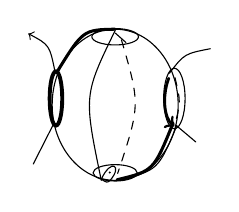
\begin{tikzpicture}[x=.8cm,y=.8cm,line cap=round]
\draw (0,0) ellipse (1 and 1.2);
\draw (0,1.08) ellipse (.37 and .13) (0,-1.08) ellipse (.35 and .13);
\draw[line width=1.4pt] (-.94,.1) ellipse (.1 and .43);
\draw (.94,.1) ellipse (.17 and .48);
\draw (.86,.5) .. controls (1.1,.81) .. (1.51,.89) (.96,-.32)--(1.28,-.59);
\draw[->] (-.95,.5)..controls (-1.04,.95)..(-1.38,1.13);
\draw (-.97,-.29)--(-1.3,-.94);
\draw (0,1.18)..controls (-.5,.15)..(-.22,-1.2);
\draw[dashed] (.1,1.03)..controls (.4,0)..(.04,-1.09);
\draw[line width=1.1pt] (-.93,.51)..controls (-.51,1.19)..(0,1.2) (.92,-.29)..controls (.61,-1.05)..(.03,-1.19);
\draw (0,1.14)--(.17,.99);
\draw (-.22,-1.18) .. controls (-.06,-.84) and (.12,-.97) .. (-.08,-1.2)
 .. controls (-.13,-1.24) .. (-.22,-1.18);
\fill (-.085,-1.075) circle (.018);
\draw[dashed] (.95,.43) .. controls (1.04,.05) .. (.95,-.31);
\draw[->,line width=1pt] (.85,.42) .. controls (.74,.12) and (.78,-.22) .. (.94,-.34);
\draw (.98,-.33) .. controls (.68,-1.04) .. (.04,-1.2);
\end{tikzpicture}}
\figure{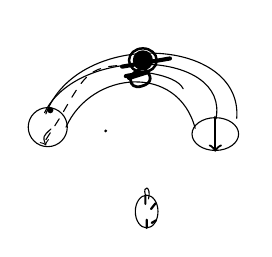
\begin{tikzpicture}[x=.8cm,y=.8cm,line cap=round]
\draw (-1.4,-.1) .. controls (-.89,1.26) and (1.73,1.13) .. (1.63,-.17);
\draw (-1.42,-.08) .. controls (-.89,1) and (1.52,.92) .. (1.3,-.18);
\draw (-1.08,-.31) .. controls (-.68,.59) and (.7,.71) .. (.97,-.33);
\draw (-1.37,-.31) circle (.31) (1.29,-.42) ellipse (.37 and .26);
\draw[->,line width=.8pt] (1.29,-.15)--(1.29,-.7);
\draw[dashed] (-1.4,-.51)--(-1.17,-.15)..controls (-.7,.67)..(.22,.68);
\fill (.14,.75) circle (.16);
\draw[line width=.9pt] (.14,.75) ellipse (.22 and .19);
\draw[line width=1pt] (.16,.62) .. controls (-.14,.58) and (-.1,.27) .. (.12,.34)
 .. controls (.31,.39) and (.28,.52) .. (.16,.62);
\draw (.24,.55) .. controls (.53,.5) and (.72,.42) .. (.78,.3);
\draw[->] (-1.32,-.34) .. controls (-1.45,-.46) .. (-1.4,-.6);
\draw[line width=1.5pt] (-.19,.65)--(.57,.78) (-.08,.47)--(.24,.57)--(-.13,.5);
\fill (-1.33,-.04) circle (.05);
\fill (-.45,-.37) circle (.025);
\draw (.2,-1.65) ellipse (.18 and .26);
\draw (.18,-1.39) .. controls (.13,-1.22) and (.28,-1.24) .. (.23,-1.45);
\draw[line width=.8pt] (.18,-1.4)--(.18,-1.53)
 (.34,-1.52)--(.27,-1.61) (.35,-1.79)--(.28,-1.83)
 (.2,-1.91)--(.2,-1.78);
\end{tikzpicture}}
\margin{Justine}% written upside down in the lower-left margin
\margin{26}

\scanpage{28}
\figure{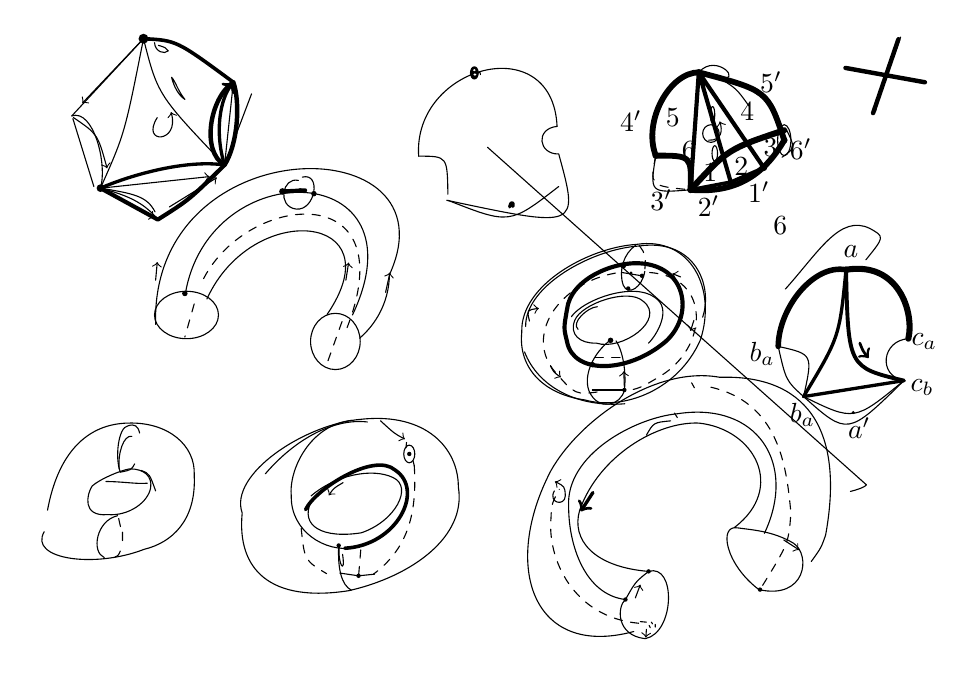
\begin{tikzpicture}[x=.007cm,y=-.007cm,line cap=round,line join=round]
\begin{scope}[shift={(246,60)}]
\draw[line width=1.3pt] (0,0) .. controls (60,3) .. (163,79);
\draw (0,0)--(-130,140) (0,0) .. controls (-34,172) .. (-78,271);
\draw (0,0) .. controls (26,102) .. (147,229);
\draw (-130,140) .. controls (-91,127) and (-65,226) .. (-78,271);
\draw (-128,145)--(-90,268);
\draw[line width=1.6pt] (163,79) .. controls (120,107) and (104,205) .. (147,229) .. controls (171,191) and (176,117) .. (163,79);
\draw (163,79)--(147,229);
\draw[line width=1.2pt] (-78,271) .. controls (-18,245) and (80,219) .. (147,229);
\draw[line width=1.5pt] (-78,271)--(26,328) .. controls (83,292) .. (147,229);
\draw (-78,271) .. controls (-29,284) and (1,297) .. (26,328);
\draw (-78,271) .. controls (-18,281) and (6,285) .. (21,314);
\draw[->] (-77,271)--(120,250);
\draw[->] (0,0)--(-111,117);
\draw[->] (-127,143) .. controls (-83,173) .. (-66,235);
\draw[->] (25,143) .. controls (-6,192) and (66,190) .. (50,133);
\fill (0,0) circle (9); \fill (-78,271) circle (7);
\draw (20,7) .. controls (21,24) and (38,29) .. (45,22) .. controls (40,16) .. (27,12);
\draw (51,70) .. controls (58,77) and (62,94) .. (75,110) .. controls (64,103) and (55,87) .. (51,70);
\draw (196,100)--(147,229);
\draw[->,line width=1.2pt] (147,229) .. controls (129,171) and (138,110) .. (163,79);
\draw[->] (-39,294)--(20,324);
\draw[->] (47,305)--(133,252);
\end{scope}
\begin{scope}[shift={(877,251)}]
\draw (-132,22) .. controls (-143,-142) and (111,-210) .. (119,-32);
\draw (119,-32) .. controls (79,-28) and (85,19) .. (122,18) .. controls (159,153) .. (-81,102);
\draw (-132,22) .. controls (-80,22) .. (-79,91);
\draw (-79,102) .. controls (33,146) .. (122,77);
\fill (-31,-129) ellipse (8 and 12);
\fill[white] (-31,-134) ellipse (2.5 and 2) (-30,-126) ellipse (2.7 and 2.2);
\draw (-25,-128) .. controls (-21,-132) .. (-20,-126);
\draw[line width=1.2pt] (33,114) .. controls (35,103) and (41,105) .. (39,113);
\end{scope}
\begin{scope}[shift={(1253,121)}]
\draw[line width=2.1pt] (0,0) .. controls (-53,0) and (-102,89) .. (-78,151) .. controls (-13,151) .. (-15,213) .. controls (66,220) and (118,187) .. (155,123) .. controls (125,33) .. (0,0);
\draw (-78,151) .. controls (-89,219) .. (-15,213);
\draw[line width=2.2pt] (-15,213) .. controls (53,139) .. (155,105);
\draw[line width=1.5pt] (0,0)--(-15,213) (0,0)--(118,173) (0,0)--(58,199);
\draw (0,0) .. controls (32,-37) and (84,20) .. (35,9) .. controls (68,29) .. (91,61);
\draw[line width=1.3pt] (-15,213)--(58,199)--(118,173);
\draw (155,123) ellipse (12 and 28);
\draw (-78,151) .. controls (-9,152) .. (-15,213);
\draw[dashed] (-78,151) .. controls (-89,206) .. (-15,213);
\draw (25,77) ellipse (4 and 15);
\draw (22,111) ellipse (15 and 16);
\draw (29,147) ellipse (5 and 14);
\draw[->] (18,123) .. controls (42,124) and (43,105) .. (38,89);
\draw (159,104) .. controls (175,137) .. (151,154);
\foreach \x/\y in {0/0,-78/151,-15/213,118/173,155/123}{\fill (\x,\y) circle (6);}
\node at (21,181) {\(\unsure{1}\)};
\node at (77,171) {\(2\)};
\node at (130,136) {\(3\)};
\node at (88,72) {\(4\)};
\node at (-47,82) {\(5\)};
\node at (-18,142) {\(6\)};
\node at (109,218) {\(1'\)};
\node at (18,243) {\(2'\)};
\node at (-68,232) {\(3'\)};
\node at (-123,89) {\(4'\)};
\node at (131,17) {\(5'\)};
\node at (185,140) {\(6'\)};
\node at (148,278) {\(6\)};
\end{scope}
\draw[line width=1.6pt] (1519,113)--(1663,139) (1615,61)--(1569,195);
\draw (1619,57)--(1606,95) (1576,174)--(1574,191);
\begin{scope}[shift={(486,468)}]
\draw (-218,110) .. controls (-228,-250) and (330,-250) .. (206,20) .. controls (205,72) and (180,111) .. (152,135);
\draw (-164,54) .. controls (-120,-203) and (273,-190) .. (139,93);
\draw (-125,64) .. controls (-42,-118) and (218,-91) .. (93,92);
\draw[dashed] (-131,27) .. controls (-48,-132) and (240,-155) .. (126,124);
\draw (-162,93) ellipse (58 and 43);
\draw (108,141) ellipse (45 and 51);
\draw[dashed] (-148,73)--(-165,133) (120,105)--(91,186);
\draw (41,-151) .. controls (12,-158) and (1,-104) .. (37,-99) .. controls (72,-96) and (83,-166) .. (48,-157);
\draw[line width=1.5pt] (12,-131)--(53,-133);
\fill (12,-131) circle (6);
\fill (-165,54) circle (5);
\fill (44,-133) circle (4) (69,-127) circle (5);
\draw[->] (-218,30)--(-215,-3);
\draw[->] (127,30)--(132,-2);
\draw[->] (199,52)--(207,16);
\end{scope}
\begin{scope} % A28-middle_ring
\draw (932,592) .. controls (929,506) and (1055,438) .. (1140,433) .. controls (1238,418) and (1286,513) .. (1256,606) .. controls (1216,697) and (1117,735) .. (1046,715) .. controls (973,705) and (925,658) .. (932,592);
\draw (939,582) .. controls (938,507) and (1062,441) .. (1144,436) .. controls (1247,421) and (1279,509) .. (1260,565);
\draw (937,628) .. controls (962,692) and (1033,729) .. (1119,722);
\draw[line width=1.5pt] (1014,551) .. controls (1020,495) and (1103,461) .. (1154,468) .. controls (1233,478) and (1243,564) .. (1193,609) .. controls (1125,667) and (1025,670) .. (1014,609) .. controls (1008,585) .. (1014,551);
\draw (1028,571) .. controls (1039,541) and (1125,511) .. (1152,536) .. controls (1195,569) and (1114,627) .. (1067,612) .. controls (1037,613) and (1018,596) .. (1028,571);
\draw (1022,564) .. controls (1045,532) and (1135,501) .. (1173,529) .. controls (1206,550) and (1176,598) .. (1162,612);
\draw (1034,587) .. controls (1021,575) and (1051,547) .. (1069,546);
\draw[dashed] (1102,485) .. controls (997,504) and (936,600) .. (993,665) .. controls (1029,706) .. (1074,700);
\draw[dashed] (1164,484) .. controls (1277,492) and (1270,620) .. (1183,672) .. controls (1148,693) .. (1118,700);
\draw[->] (984,653) .. controls (990,665) .. (1003,674);
\draw[->] (1244,571)--(1238,590);
\draw[->] (1220,492)--(1205,486);
\draw[->] (946,572) .. controls (941,552) .. (963,549);
\draw (1138,435) .. controls (1117,450) and (1107,480) .. (1116,507) .. controls (1125,528) and (1151,510) .. (1155,482);
\draw[dashed] (1145,435) .. controls (1157,452) .. (1155,482);
\draw (1114,484)--(1150,490);
\fill (1116,472) circle (5) (1130,485) circle (3) (1150,490) circle (4) (1125,513) circle (4);
\draw (1092,607) .. controls (1062,630) and (1043,670) .. (1054,699) .. controls (1071,737) and (1112,725) .. (1118,697);
\draw (1103,608) .. controls (1119,633) and (1121,677) .. (1118,697);
\draw[dashed] (1065,638)--(1116,638);
\draw (1060,697)--(1118,697);
\draw[->] (1118,691)--(1117,663);
\fill (1093,607) circle (5) (1060,651) circle (5) (1118,697) circle (4);
\end{scope}
\draw (870,257)--(1557,869) .. controls (1555,873) and (1540,878) .. (1528,881);
\begin{scope}[shift={(1520,479)}]
\draw[line width=2pt] (0,0) .. controls (-59,-11) and (-122,69) .. (-123,139);
\draw[line width=2.2pt] (0,0) .. controls (96,-16) and (124,78) .. (113,125);
\draw (-123,139) .. controls (-60,153) .. (-77,230);
\draw (-123,139) .. controls (-109,201) .. (-77,230);
\draw (113,125) .. controls (65,128) and (57,192) .. (105,201);
\draw[line width=1.2pt] (0,0) .. controls (-12,122) .. (-77,230)--(105,201);
\draw[line width=1.4pt] (0,0) .. controls (4,177) .. (105,201);
\draw[->,line width=1pt] (25,133) .. controls (31,148) .. (41,160);
\draw (-77,230) .. controls (3,301) .. (105,201);
\draw (-77,230) .. controls (15,275) .. (105,201);
\draw (-110,35) .. controls (-49,-33) and (-11,-101) .. (43,-75) .. controls (70,-60) .. (36,-18);
\fill (0,0) circle (6);
\fill (13,259) circle (3);
\node at (9,-33) {\(a\)};
\node at (-152,152) {\(b_a\)};
\node at (-79,263) {\(b_a\)};
\node at (142,130) {\(c_a\)};
\node at (138,214) {\(c_b\)};
\node at (24,287) {\(a'\)};
\end{scope}
\begin{scope} % A28-lower_left_torus
\draw (72,915) .. controls (91,811) and (144,758) .. (219,757) .. controls (290,755) and (341,797) .. (338,852) .. controls (342,934) and (297,974) .. (247,986) .. controls (157,1021) and (37,1004) .. (66,954);
\draw (153,871) .. controls (143,886) and (134,927) .. (181,923) .. controls (220,926) and (255,900) .. (259,874) .. controls (262,854) and (248,840) .. (221,840) .. controls (204,843) and (168,858) .. (153,871);
\draw (242,843) .. controls (257,849) .. (268,880);
\draw (204,846) .. controls (194,821) and (200,764) .. (218,762) .. controls (230,758) and (236,762) .. (239,775);
\draw (202,840) .. controls (199,812) and (210,778) .. (225,781);
\draw (204,846) .. controls (224,842) .. (230,831);
\draw (199,925) .. controls (160,934) and (151,991) .. (175,1001);
\draw[dashed] (201,930)--(205,948) (208,955)--(208,973) (204,989) .. controls (200,998) .. (193,1000);
\draw (178,863) .. controls (208,863) and (235,868) .. (253,866);
\end{scope}
\begin{scope} % A28-lower_middle_ring
\draw (425,920) .. controls (400,850) and (539,758) .. (642,750) .. controls (758,738) and (817,802) .. (817,873) .. controls (832,963) and (733,1035) .. (618,1061) .. controls (476,1083) and (415,1023) .. (425,920);
\draw (467,849) .. controls (522,785) and (592,748) .. (652,755);
\draw (550,889) .. controls (593,852) and (660,837) .. (699,856) .. controls (735,873) and (703,935) .. (641,956) .. controls (571,967) and (529,944) .. (550,899);
\draw[line width=1.3pt] (540,914) .. controls (557,877) and (664,809) .. (702,842) .. controls (757,878) and (706,979) .. (611,984);
\draw (624,752) .. controls (549,760) and (509,840) .. (514,890) .. controls (513,952) and (574,993) .. (630,983);
\draw[dashed] (532,948) .. controls (538,1006) .. (578,1030);
\draw[dashed] (737,834) .. controls (743,927) and (722,987) .. (663,1031);
\draw (600,979) .. controls (598,1021) and (605,1051) .. (623,1060);
\draw[dashed] (640,987)--(636,1035);
\draw (602,1029)--(636,1034)--(665,1031);
\draw (601,982) .. controls (598,1014) and (613,1034) .. (607,995);
\fill (600,979) circle (4) (636,1034) circle (4);
\draw (728,813) ellipse (10 and 16);
\fill (728,813) circle (4);
\draw (723,792)--(722,802) (735,826)--(737,834);
\draw[->] (676,753) .. controls (701,776) .. (720,786);
\draw[->] (608,865) .. controls (591,875) .. (582,888);
\end{scope}
\begin{scope} % A28-lower_handle
\draw (1135,1135) .. controls (950,1185) and (895,1015) .. (985,843) .. controls (1039,748) and (1177,653) .. (1291,674) .. controls (1443,669) and (1519,762) .. (1483,960) .. controls (1475,983) .. (1457,1008);
\draw (1120,1077) .. controls (1046,1068) and (1017,978) .. (1017,909) .. controls (1011,814) and (1138,747) .. (1215,740) .. controls (1359,718) and (1432,830) .. (1372,957);
\draw (1162,1026) .. controls (1063,1018) and (1021,969) .. (1037,915) .. controls (1072,816) and (1178,754) .. (1253,757) .. controls (1355,768) and (1411,875) .. (1318,946);
\draw (1162,1026) .. controls (1212,1011) and (1210,1137) .. (1156,1148) .. controls (1102,1142) and (1105,1089) .. (1120,1077) .. controls (1138,1045) .. (1162,1026);
\draw (1323,947) .. controls (1289,941) and (1300,1012) .. (1362,1059) .. controls (1447,1078) and (1457,997) .. (1425,975) .. controls (1388,953) and (1352,951) .. (1323,947);
\draw[dashed] (1144,1120) .. controls (1025,1109) and (978,1003) .. (985,929) .. controls (986,904) .. (1000,877);
\draw[dashed] (1275,692) .. controls (1396,720) and (1412,830) .. (1420,920) .. controls (1416,975) .. (1364,1059);
\draw[->,line width=1.2pt] (1061,883)--(1039,917);
\draw[->] (1407,969)--(1435,987);
\draw[->] (1138,1074)--(1147,1050);
\draw[->] (991,880) .. controls (979,902) and (1010,909) .. (1011,889) .. controls (1010,872) .. (992,863);
\draw (1147,1117)--(1158,1118) (1167,1118)--(1169,1121) (1174,1122)--(1174,1127) (1163,1124)--(1165,1128);
\draw[->] (1158,1131)--(1157,1146);
\draw (1240,684)--(1245,693) (1209,739)--(1214,747);
\draw (1158,779) .. controls (1171,756) .. (1202,753);
\fill (1162,1026) circle (4) (1120,1077) circle (4) (1364,1059) circle (4);
\end{scope}
\end{tikzpicture}}% crop-candidate: scan 28
\begin{gather*}
4\text{ sommets}\\6\text{ arêtes}\\2\text{ \unsure{hexagones|triangles}}
\end{gather*}
\margin{27}

\cotefile{148}
\scanpage{29}
\margin{\(M_{0,5}\;\unsure{-}\)}

\margin{28}

\scanpage{31}
\margin{\figure{\begin{tikzpicture}[x=1cm,y=1cm]\draw (.12,.32)--(.1,.08)..controls(.09,.01)and(.02,.01)..(0,.05);\end{tikzpicture}}}
\margin{\figure{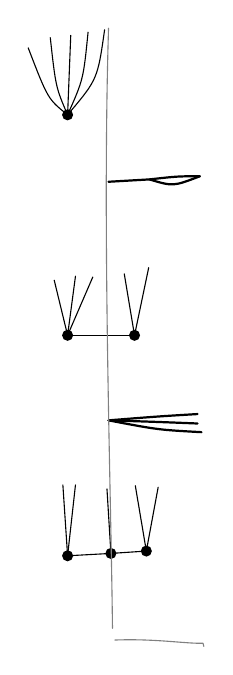
\begin{tikzpicture}[x=1cm,y=1cm,line cap=round,line join=round]
\fill (0,6.2) circle(2pt);
\draw (0,6.2)..controls(-.25,6.4)..(-.5,7.05);
\draw (0,6.2)..controls(-.15,6.55)..(-.22,7.18);
\draw (0,6.2)--(.04,7.21);
\draw (0,6.2)..controls(.2,6.65)..(.26,7.25);
\draw (0,6.2)..controls(.38,6.65)..(.47,7.28);
\draw (0,3.4)--(.85,3.4);\fill (0,3.4) circle(2pt);\fill (.85,3.4) circle(2pt);
\draw (0,3.4)--(-.17,4.1);\draw (0,3.4)--(.1,4.15);\draw (0,3.4)--(.32,4.14);
\draw (.85,3.4)--(.72,4.18);\draw (.85,3.4)--(1.03,4.26);
\draw (0,.6)--(.55,.63)--(1,.66);
\foreach \x/\y in {0/.6,.55/.63,1/.66}{\fill (\x,\y) circle(2pt);}
\draw (0,.6)--(-.06,1.5);\draw (0,.6)--(.1,1.5);\draw (.55,.63)--(.5,1.45);\draw (1,.66)--(.86,1.49);\draw (1,.66)--(1.15,1.47);
% Literal courses of the two retraced marginal arrows.
\draw[thick] (.52,5.35)--(1.04,5.38)..controls(1.4,5.42)..(1.68,5.42);
\draw[thick] (1.68,5.42)..controls(1.34,5.29)..(1.04,5.38);
\draw[thick] (.52,2.32)..controls(1.15,2.37)..(1.65,2.4);
\draw[thick] (.52,2.32)..controls(1.15,2.3)..(1.65,2.28);
\draw[thick] (.52,2.32)..controls(1.15,2.2)..(1.7,2.17);
\draw[gray] (.52,7.3)..controls(.44,4.7)and(.55,1.5)..(.57,-.32);
\draw[gray] (.6,-.47)..controls(1.12,-.45)and(1.52,-.52)..(1.72,-.51)--(1.73,-.55);
\end{tikzpicture}}}


\diagram{\begin{tikzcd}[ampersand replacement=\&,column sep=9em,row sep=10em]
\begin{gathered}\mathrm{I}_{10}\ (\text{pentagonale})\\
\vcenter{\hbox{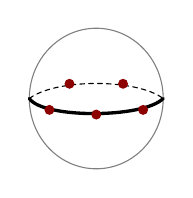
\begin{tikzpicture}[x=.85cm,y=.85cm,line cap=round,line join=round]
\draw[gray] (0,0) ellipse (1 and 1.05);
\draw[very thick] (-1,0)..controls(-.8,-.3)and(.7,-.3)..(1,0);
\draw[dash pattern=on 1.7pt off 1.5pt] (-1,0)..controls(-.6,.3)and(.6,.3)..(1,0);
\fill[red!55!black] (-.7,-.17) circle(1.8pt);
\fill[red!55!black] (0,-.24) circle(1.8pt);
\fill[red!55!black] (.7,-.17) circle(1.8pt);
\fill[red!55!black] (-.4,.22) circle(1.8pt);
\fill[red!55!black] (.4,.22) circle(1.8pt);
\end{tikzpicture}}}\\
\text{12 structures pentagonales sur }K\\
\{\sigma,\sigma^{-1}\}\in P_2(\mathrm{Circ}(K)\\
G\simeq\mathbb D_5\\
\widetilde G\simeq\mathbb D_5\times\{1,\sigma\}\end{gathered}\&\begin{gathered}\mathrm I_6\ (\text{bitétraédrale})\\
\vcenter{\hbox{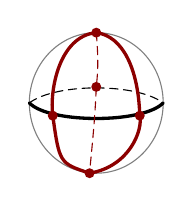
\begin{tikzpicture}[x=.85cm,y=.85cm,line cap=round,line join=round]
\draw[gray] (0,0) ellipse (1 and 1.05);
\draw[very thick] (-1,0)..controls(-.7,-.31)and(.7,-.31)..(1,0);
\draw[densely dashed] (-1,0)..controls(-.6,.3)and(.6,.3)..(1,0);
\draw[red!55!black,very thick] (0,1.05)..controls(-.55,1)and(-.7,.2)..(-.65,-.19)..controls(-.55,-.9)..(-.1,-1.05)..controls(.5,-.95)and(.7,-.4)..(.65,-.19)..controls(.63,.5)and(.4,1)..(0,1.05);
\draw[red!55!black,densely dashed] (0,1.05)..controls(.03,.7)and(.03,.5)..(0,.24)..controls(-.02,-.3)and(-.08,-.8)..(-.1,-1.05);
\fill[red!55!black] (0,1.05) circle(1.8pt);
\fill[red!55!black] (-.65,-.19) circle(1.8pt);
\fill[red!55!black] (.65,-.19) circle(1.8pt);
\fill[red!55!black] (0,.24) circle(1.8pt);
\fill[red!55!black] (-.1,-1.05) circle(1.8pt);
\end{tikzpicture}}}\\
\text{20 structures }K=J\amalg\omega\\
\text{avec }\omega\xrightarrow{\sim}\underline\omega(J)\\
G\simeq\unsure{\mathfrak S|G}_J\simeq\unsure{\mathfrak S|G}_3\\
\widetilde G\simeq\unsure{\mathfrak S|G}_3\times\{1,\sigma\}\end{gathered} \arrow[r,"{3\quad f_{B,s}\quad2}","{(B\in\unsure{\mathrm{Bit\acute et}|\mathrm{Bitet}}(K),\ s\in T(B)=J)}"'] \& \begin{gathered}\mathrm I_4\ (\text{pyramidale})\\
\vcenter{\hbox{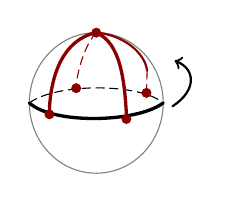
\begin{tikzpicture}[x=.85cm,y=.85cm,line cap=round,line join=round]
\draw[gray] (0,0) ellipse (1 and 1.05);
\draw[very thick] (-1,0)..controls(-.65,-.32)and(.6,-.3)..(1,0);
\draw[densely dashed] (-1,0)..controls(-.6,.3)and(.65,.3)..(1,0);
\draw[red!55!black,very thick] (0,1.05)..controls(-.5,.95)and(-.68,.4)..(-.7,-.10);
\draw[red!55!black,very thick] (0,1.05)..controls(.36,.9)and(.42,.35)..(.45,-.16);
\draw[red!55!black,densely dashed] (0,1.05)..controls(-.15,.9)and(-.29,.5)..(-.3,.22);
\draw[red!55!black,thick] (0,1.05)..controls(.4,1.02)and(.73,.75)..(.76,.48);
\draw[red!55!black,densely dashed] (.76,.48)--(.75,.15);
\draw[->,thick] (1.14,-.05)..controls(1.52,.2)and(1.47,.52)..(1.17,.63);
\fill[red!55!black] (0,1.05) circle(1.8pt);
\fill[red!55!black] (-.7,-.17) circle(1.8pt);
\fill[red!55!black] (.45,-.24) circle(1.8pt);
\fill[red!55!black] (-.3,.22) circle(1.8pt);
\fill[red!55!black] (.75,.15) circle(1.8pt);
\end{tikzpicture}}}\\
\text{30 structures carrés orientés}\\
K\simeq\{P\}\amalg I\\
I\ \text{structure carrée \uline{orientée}}\ (Q,\omega)=\vec Q\\
I=\coprod_{\alpha\in\delta}\alpha\qquad\delta=\text{ens. des diagonales }\alpha\\
\omega\in\delta\wedge\bigwedge_{\alpha\in\delta}\alpha\\
G=\widetilde G=\mathbb Z/4\mathbb Z\end{gathered} \arrow[dl,bend right=10,pos=.27,"{4\quad f_{\vec Q,\omega,a}\quad2}","{(Q=\overrightarrow{\mathrm{Carr}}(K),\ a\in\Lambda(Q))}"'] \\
\begin{gathered}\mathrm{II}_2\ (\text{carré-triangle droit})\\
\vcenter{\hbox{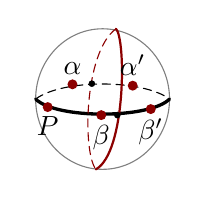
\begin{tikzpicture}[x=.85cm,y=.85cm,line cap=round,line join=round]
\draw[gray] (0,0) ellipse (1 and 1.05);
\draw[very thick] (-1,0)..controls(-.7,-.3)and(.7,-.3)..(1,0);
\draw[densely dashed] (-1,0)..controls(-.6,.3)and(.6,.3)..(1,0);
\draw[red!55!black,thick] (.2,1.05)..controls(.35,.9)and(.35,-.8)..(-.1,-1.05);
\draw[red!55!black,densely dashed] (.2,1.05)..controls(-.28,.7)and(-.3,-.8)..(-.1,-1.05);
\fill[red!55!black] (-.45,.22) circle(1.8pt) node[above,black] {$\alpha$};
\fill[red!55!black] (.45,.2) circle(1.8pt) node[above,black] {$\alpha'$};
\fill[red!55!black] (-.82,-.12) circle(1.8pt) node[below,black] {$P$};
\fill[red!55!black] (-.02,-.24) circle(1.8pt) node[below,black] {$\beta$};
\fill[red!55!black] (.72,-.15) circle(1.8pt) node[below,black] {$\beta'$};
\fill (-.16,.23) circle(1.2pt);\fill (.22,-.24) circle(1.2pt);
\end{tikzpicture}}}\\
\text{2 sommets-repères}\quad\deleted{\text{\unsure{repères}}}\\
\text{60 structures ``pentagone}\\
\text{avec sommet'' sur }K\\
\text{i.e. }K\simeq B\amalg\omega,\ \text{avec }\omega\hookrightarrow J\\
\text{i.e. }P\in J\text{ et }\omega\simeq\omega'=B\setminus\{P\}\\
G\simeq\mathbb Z/2\mathbb Z\\
\widetilde G\simeq\mathbb Z/2\mathbb Z\times\{1,\sigma\}\end{gathered} \arrow[u,"{1\quad\gamma_{\pi,s}\quad5}","{(\pi\in\mathrm{Pent}(K),\ s\in K)}"'] \arrow[r,"{1\quad\tau_{\pi,s}=\mathrm{tw}_{1/4}\quad1}"] \& \begin{gathered}\mathrm{II}'_2=\mathrm{Tw}_{1/4}\mathrm{II}_2\\
(\text{carré-triangle gauche})\\
\text{4 sommets}\ \deleted{\text{\unsure{repères}}}\\
\vcenter{\hbox{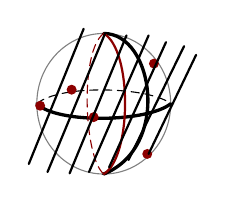
\begin{tikzpicture}[x=.85cm,y=.85cm,line cap=round,line join=round]
% The drawing is canceled by its seven oblique strokes. No alphabetic labels are secure beneath them.
\draw[gray] (0,0) ellipse (1 and 1.05);
\draw[very thick] (0,1.05)..controls(.75,1.05)and(1,-.65)..(0,-1.05);
\draw[very thick] (-1,0)..controls(-.7,-.3)and(.65,-.28)..(1,0);
\draw[densely dashed] (-1,0)..controls(-.65,.3)and(.7,.25)..(1,0);
\draw[red!55!black,thick] (0,1.05)..controls(.43,.8)and(.42,-.8)..(0,-1.05);
\draw[red!55!black,densely dashed] (0,1.05)..controls(-.36,.8)and(-.3,-.8)..(0,-1.05);
\fill[red!55!black] (-.95,-.03) circle(1.8pt);
\fill[red!55!black] (-.48,.21) circle(1.8pt);
\fill[red!55!black] (-.15,-.2) circle(1.8pt);
\fill[red!55!black] (.75,.6) circle(1.8pt);
\fill[red!55!black] (.65,-.75) circle(1.8pt);
\draw[thick] (-1.12,-.9)--(-.3,1.12);
\draw[thick] (-.84,-1.02)--(.02,1.05);
\draw[thick] (-.51,-1.04)--(.34,1.02);
\draw[thick] (-.22,-1.02)--(.67,1.02);
\draw[thick] (.08,-.95)--(.93,.92);
\draw[thick] (.37,-.84)--(1.2,.86);
\draw[thick] (.67,-.75)--(1.38,.73);
\end{tikzpicture}}}\quad\vcenter{\hbox{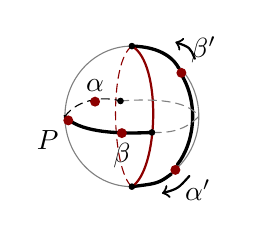
\begin{tikzpicture}[x=.85cm,y=.85cm,line cap=round,line join=round]
\draw[gray] (0,0) ellipse (1 and 1.05);
\draw[very thick] (0,1.05)..controls(.46,1.04)and(.64,.84)..(.7,.72);
\draw[very thick] (.76,.59)..controls(1,.16)and(.93,-.4)..(.68,-.72);
\draw[very thick] (.59,-.86)..controls(.4,-1)..(0,-1.05);
\draw[red!55!black,thick] (0,1.05)..controls(.45,.8)and(.4,-.8)..(0,-1.05);
\draw[red!55!black,densely dashed] (0,1.05)..controls(-.35,.8)and(-.3,-.8)..(0,-1.05);
\draw[very thick] (-1,0)..controls(-.8,-.22)and(-.3,-.27)..(.3,-.24);
\draw[densely dashed] (-1,0)..controls(-.8,.27)and(-.4,.3)..(-.17,.23);
\draw[gray,densely dashed] (-.17,.23)..controls(.48,.28)and(.86,.2)..(1,0)..controls(.8,-.2)and(.6,-.25)..(.3,-.24);
\fill[red!55!black] (-.55,.22) circle(1.8pt) node[above,black] {$\alpha$};
\fill[red!55!black] (.74,.65) circle(1.8pt) node[above right,black] {$\beta'$};
\fill[red!55!black] (-.95,-.06) circle(1.8pt) node[below left,black] {$P$};
\fill[red!55!black] (-.15,-.25) circle(1.8pt) node[below,black] {$\beta$};
\fill[red!55!black] (.65,-.8) circle(1.8pt) node[below right,black] {$\alpha'$};
\fill (0,1.05) circle(1.2pt);\fill (0,-1.05) circle(1.2pt);\fill (-.17,.23) circle(1.2pt);\fill (.3,-.24) circle(1.2pt);
\draw[->,thick] (.94,.86)..controls(.87,1.03)..(.65,1.11);
\draw[->,thick] (.86,-.89)..controls(.69,-1.08)..(.45,-1.15);
\end{tikzpicture}}}\\
\text{même paramétrage que }\mathrm{II}_2\\
G\simeq\mathbb Z/2\mathbb Z,\ \widetilde G\simeq\mathbb Z/2\mathbb Z\times\{1,\sigma\}\end{gathered} \arrow[u,"{\gamma'_{\pi,s}\quad3}","{\text{comp. avec }\unsure{\vec Q|\vec G};\ (\pi\in\mathrm{Pent}(K),\ s\in K)}"'] \& \begin{gathered}\mathrm{II}_1\ (\text{tétraèdre-triangle})\\
\vcenter{\hbox{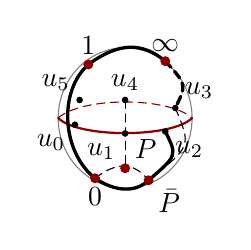
\begin{tikzpicture}[x=.85cm,y=.85cm,line cap=round,line join=round]
\draw[gray] (0,0) ellipse (1 and 1.05);
\draw[red!55!black,thick] (-1,0)..controls(-.7,-.3)and(.7,-.3)..(1,0);
\draw[red!55!black,densely dashed] (-1,0)..controls(-.65,.32)and(.65,.32)..(1,0);
\draw[very thick] (-.55,.8)..controls(-1,.4)and(-.95,-.5)..(-.45,-.9);
\draw[very thick] (-.55,.8)..controls(-.1,1.13)and(.25,1.14)..(.6,.85);
\draw[very thick,densely dashed] (.6,.85)..controls(.92,.5)..(.75,.15);
\draw[densely dashed] (.75,.15)..controls(.99,-.42)..(.35,-.93);
\draw[very thick] (.6,-.2)..controls(.78,-.56)..(.35,-.93);
\draw[very thick] (-.45,-.9)..controls(-.15,-1.1)and(.15,-1.12)..(.35,-.93);
\draw[densely dashed] (-.45,-.9)..controls(-.12,-.65)and(.12,-.65)..(.35,-.93);
\draw[densely dashed] (0,.27)--(0,-.75);
\fill[red!55!black] (-.55,.8) circle(1.8pt) node[above,black] {$1$};
\fill[red!55!black] (.6,.85) circle(1.8pt) node[above,black] {$\infty$};
\fill[red!55!black] (-.45,-.9) circle(1.8pt) node[below,black] {$0$};
\fill[red!55!black] (.35,-.93) circle(1.8pt) node[below right,black] {$\unsure{\bar P}$};
\fill[red!55!black] (0,-.75) circle(1.8pt) node[above right,black] {$\unsure{P}$};
\fill (-.75,-.1) circle(1.2pt) node[below left] {$u_0$};
\fill (0,-.23) circle(1.2pt) node[below left] {$u_1$};
\fill (.6,-.2) circle(1.2pt) node[below right] {$u_2$};
\fill (.75,.15) circle(1.2pt) node[above right] {$u_3$};
\fill (0,.27) circle(1.2pt) node[above] {$u_4$};
\fill (-.68,.27) circle(1.2pt) node[above left] {$u_5$};
\end{tikzpicture}}}\\
\text{6 sommets-repères}\\
\text{120 structures entièrement}\\
\text{épinglées,}\\
G=\deleted{\unsure{1}}=\{1\},\quad\widetilde G=\{1,\sigma\}\\
\left[\begin{gathered}K=J\amalg\varepsilon\quad\operatorname{card}J=3,\operatorname{card}\varepsilon=2\\\omega\in\underline\omega(J),\ r\in J\times\varepsilon\\\tau_r^0:\mathrm{II}_1(J,\varepsilon)\longrightarrow\mathrm{II}_1(u_\omega(r))\\\text{où }u_\omega=\omega\times(-1)\text{ sur }J\times\varepsilon\end{gathered}\right]\end{gathered} \arrow[ul,pos=.73,"{1\quad\gamma_r^0\quad6}","{\text{compat. avec }\unsure{\vec Q|\vec G}}"'] \arrow[loop right,"{\tau_r^0=\mathrm{tw}_{1/6}}"] \\
\begin{gathered}\mathrm{III}_2\ (\text{triple triangle droit})\\
\vcenter{\hbox{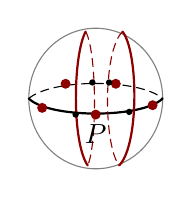
\begin{tikzpicture}[x=.85cm,y=.85cm,line cap=round,line join=round]
\draw[gray] (0,0) ellipse (1 and 1.05);
\draw[thick] (-1,0)..controls(-.7,-.3)and(.7,-.3)..(1,0);
\draw[densely dashed] (-1,0)..controls(-.65,.3)and(.65,.3)..(1,0);
\draw[red!55!black,thick] (-.15,1)..controls(-.34,.65)and(-.36,-.65)..(-.12,-1);
\draw[red!55!black,densely dashed] (-.15,1)..controls(.02,.7)and(.02,-.7)..(-.12,-1);
\draw[red!55!black,densely dashed] (.4,1)..controls(.1,.7)and(.12,-.7)..(.35,-1);
\draw[red!55!black,thick] (.4,1)..controls(.64,.7)and(.65,-.7)..(.35,-1);
\fill[red!55!black] (-.8,-.14) circle(1.8pt);
\fill[red!55!black] (0,-.24) circle(1.8pt);
\fill[red!55!black] (.85,-.1) circle(1.8pt);
\fill[red!55!black] (-.45,.22) circle(1.8pt);
\fill[red!55!black] (.3,.22) circle(1.8pt);\fill[black] (-.3,-.24) circle(1.15pt);
\fill[black] (.5,-.2) circle(1.15pt);
\fill[black] (-.05,.24) circle(1.15pt);
\fill[black] (.2,.24) circle(1.15pt);\node[below] at (0,-.25) {$P$};
\end{tikzpicture}}}\\
2+2\ \text{sommets-repère}\\
\text{60 structures ``pentagone avec}\\
\text{sommet'' sur }K,\\
G=\mathbb Z/2\mathbb Z,\widetilde G=\mathbb Z/2\mathbb Z\times\{1,\sigma\}\end{gathered} \arrow[u,start anchor=north west,"{2\quad\gamma_{\pi,\rho}\quad2}","{\begin{tikzpicture}[baseline]\draw (0,.15)..controls(-.12,.23)and(-.16,.3)..(-.14,.37);\end{tikzpicture}}"{pos=.02,description},"{(\pi\in\mathrm{Pent}(K),\rho\in\mathrm{Rep}\,\pi)}"'] \arrow[r,"{\unsure{\tau_{\pi,\omega}}}","{2\quad\tau_{\pi,\rho}=\mathrm{tw}_{1/4}\quad1}"'] \& \begin{gathered}\mathrm{III}_1\ (\text{triple triangle sem.-gauche})\\
\vcenter{\hbox{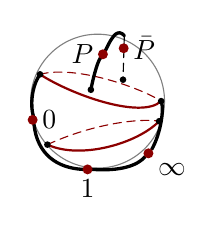
\begin{tikzpicture}[x=.85cm,y=.85cm,line cap=round,line join=round]
\draw[gray] (0,0) circle(1);
\draw[very thick] (-.86,.4)..controls(-1,.2)and(-1,-.1)..(-.96,-.22);
\draw[very thick] (-.95,-.35)..controls(-.9,-.8)and(-.6,-1)..(-.22,-1.02);
\draw[very thick] (-.08,-1.02)..controls(.35,-1.05)and(.6,-.96)..(.71,-.83);
\draw[very thick] (.81,-.72)..controls(.94,-.49)and(1,-.12)..(.95,0);
\draw[red!55!black,thick] (-.86,.4)..controls(-.4,.1)and(.65,-.28)..(.95,0);
\draw[red!55!black,densely dashed] (-.86,.4)..controls(-.35,.54)and(.6,.22)..(.95,0);
\draw[red!55!black,thick] (-.75,-.65)..controls(-.25,-.88)and(.6,-.63)..(.92,-.3);
\draw[red!55!black,densely dashed] (-.75,-.65)..controls(-.1,-.35)and(.6,-.25)..(.92,-.3);
\draw[very thick] (-.1,.17)..controls(-.05,.43)and(.02,.64)..(.05,.65);
\draw[very thick] (.12,.76)..controls(.24,1.02)and(.31,1.07)..(.4,.98);
\draw[densely dashed] (.4,.98)--(.38,.32);
\fill[red!55!black] (-.97,-.28) circle(1.8pt) node[right,black] {$0$};
\fill[red!55!black] (-.15,-1.02) circle(1.8pt) node[below,black] {$1$};
\fill[red!55!black] (.76,-.78) circle(1.8pt) node[below right,black] {$\infty$};
\fill[red!55!black] (.08,.7) circle(1.8pt) node[left,black] {$P$};
\fill[red!55!black] (.39,.79) circle(1.8pt) node[right,black] {$\bar P$};
\fill[black] (-.86,.4) circle(1.2pt);
\fill[black] (-.1,.17) circle(1.2pt);
\fill[black] (.38,.32) circle(1.2pt);
\fill[black] (.95,0) circle(1.2pt);
\fill[black] (-.75,-.65) circle(1.2pt);
\fill[black] (.92,-.3) circle(1.2pt);
\end{tikzpicture}}}\quad=\quad\vcenter{\hbox{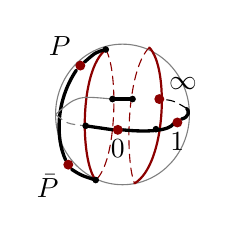
\begin{tikzpicture}[x=.85cm,y=.85cm,line cap=round,line join=round]
\draw[gray] (0,0) ellipse (1 and 1.05);
\draw[red!55!black,thick] (-.25,.97)..controls(-.65,.65)and(-.63,-.7)..(-.4,-.98);
\draw[red!55!black,densely dashed] (-.25,.97)..controls(-.06,.65)and(-.08,-.7)..(-.4,-.98);
\draw[red!55!black,densely dashed] (.4,1)..controls(.05,.65)and(.04,-.7)..(.18,-1.03);
\draw[red!55!black,thick] (.4,1)..controls(.7,.7)and(.65,-.75)..(.18,-1.03);
\draw[very thick] (-.25,.97)..controls(-.4,.93)..(-.57,.78);
\draw[very thick] (-.69,.66)..controls(-1,.2)and(-1,-.36)..(-.85,-.68);
\draw[very thick] (-.76,-.82)..controls(-.62,-.91)..(-.4,-.98);
\draw[gray,densely dashed] (-1,0)..controls(-.83,-.14)..(-.55,-.17);
\draw[very thick] (-.55,-.17)--(-.14,-.23);
\draw[very thick] (0,-.23)..controls(.4,-.27)and(.7,-.24)..(.76,-.14);
\draw[very thick] (.88,-.07)..controls(1,-.04)and(1,.05)..(.96,.09);
\draw[densely dashed] (.96,.09)..controls(.76,.21)..(.55,.23);
\draw[very thick] (-.15,.23)--(.15,.23);
\draw[gray] (-1,0)..controls(-.68,.28)..(-.15,.23);
\fill[red!55!black] (-.63,.73) circle(1.8pt) node[above left,black] {$P$};
\fill[red!55!black] (-.81,-.75) circle(1.8pt) node[below left,black] {$\bar P$};
\fill[red!55!black] (-.07,-.23) circle(1.8pt) node[below,black] {$0$};
\fill[red!55!black] (.82,-.12) circle(1.8pt) node[below,black] {$1$};
\fill[red!55!black] (.55,.23) circle(1.8pt) node[above right,black] {$\infty$};
\fill[black] (-.25,.97) circle(1.2pt);
\fill[black] (-.4,-.98) circle(1.2pt);
\fill[black] (-.55,-.17) circle(1.2pt);
\fill[black] (-.15,.23) circle(1.2pt);
\fill[black] (.15,.23) circle(1.2pt);
\fill[black] (.5,-.22) circle(1.2pt);
\end{tikzpicture}}}\\
\text{2+4 sommets-repère}\\
\text{120 structures épinglées}\\
G=1,\widetilde G=\{1,\sigma\}\end{gathered} \arrow[u,"{1\quad\gamma_r^1\quad2}"] \arrow[ur,"{3\qquad3}","{(r\in\mathrm{Rep}(K))}"',"{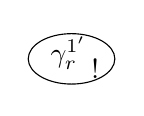
\begin{tikzpicture}[baseline=-.6ex]\draw (0,0) ellipse (.55 and .32);\node at (-.04,.07) {$\gamma_r^{1'}$};\node at (.3,-.13) {$!$};\end{tikzpicture}}"{description}] \arrow[r,"{1\quad\tau'_r\quad2}"] \& \begin{gathered}\mathrm{III}'_2\ (\text{triple triangle gauche})\\
\vcenter{\hbox{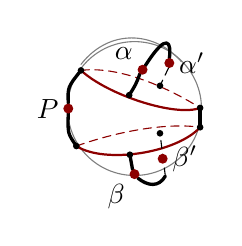
\begin{tikzpicture}[x=.85cm,y=.85cm,line cap=round,line join=round]
\draw[gray] (0,0) circle(1);
\draw[gray] (-.8,.66)..controls(-.38,1.2)and(.3,1.16)..(.7,.7);
\draw[very thick] (-.8,.57)..controls(-1,.32)..(-.99,.08);
\draw[very thick] (-.99,-.07)..controls(-1,-.37)..(-.87,-.56);
\draw[very thick] (.98,.01)--(.98,-.28);
\draw[red!55!black,thick] (-.8,.57)..controls(-.4,.2)and(.62,-.13)..(.98,.01);
\draw[red!55!black,densely dashed] (-.8,.57)..controls(-.15,.65)and(.65,.22)..(.98,.01);
\draw[red!55!black,thick] (-.87,-.56)..controls(-.45,-.83)and(.62,-.67)..(.98,-.28);
\draw[red!55!black,densely dashed] (-.87,-.56)..controls(-.1,-.29)and(.58,-.22)..(.98,-.28);
\draw[very thick] (-.08,.2)..controls(.02,.36)..(.08,.52);
\draw[very thick] (.16,.64)..controls(.5,1.17)and(.55,.98)..(.52,.75);
\draw[densely dashed] (.51,.61)--(.38,.34);
\draw[very thick] (-.07,-.69)--(-.03,-.91);
\draw[very thick] (.05,-1.04)..controls(.2,-1.16)and(.36,-1.18)..(.46,-1.01);
\draw[densely dashed] (.46,-1.01)--(.38,-.37);
\fill[red!55!black] (-.99,0) circle(1.8pt) node[left,black] {$P$};
\fill[red!55!black] (.12,.58) circle(1.8pt) node[above left,black] {$\alpha$};
\fill[red!55!black] (.52,.68) circle(1.8pt) node[right,black] {$\unsure{\alpha'}$};
\fill[red!55!black] (0,-.98) circle(1.8pt) node[below left,black] {$\unsure{\beta}$};
\fill[red!55!black] (.42,-.75) circle(1.8pt) node[right,black] {$\unsure{\beta'}$};
\fill[black] (-.8,.57) circle(1.2pt);
\fill[black] (-.08,.2) circle(1.2pt);
\fill[black] (.38,.34) circle(1.2pt);
\fill[black] (.98,.01) circle(1.2pt);
\fill[black] (-.87,-.56) circle(1.2pt);
\fill[black] (-.07,-.69) circle(1.2pt);
\fill[black] (.38,-.37) circle(1.2pt);
\fill[black] (.98,-.28) circle(1.2pt);
\end{tikzpicture}}}\quad\simeq\quad\vcenter{\hbox{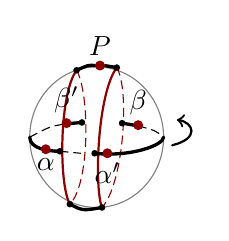
\begin{tikzpicture}[x=.85cm,y=.85cm,line cap=round,line join=round]
\draw[gray] (0,0) ellipse (1 and 1.05);
\draw[red!55!black,thick] (-.3,1)..controls(-.56,.65)and(-.57,-.7)..(-.4,-1);
\draw[red!55!black,densely dashed] (-.3,1)..controls(-.1,.65)and(-.1,-.7)..(-.4,-1);
\draw[red!55!black,thick] (.3,1.04)..controls(.01,.65)and(-.04,-.75)..(.08,-1.05);
\draw[red!55!black,densely dashed] (.3,1.04)..controls(.5,.7)and(.4,-.7)..(.08,-1.05);
\draw[very thick] (-.3,1)..controls(-.12,1.08)..(-.02,1.07);
\draw[very thick] (.12,1.07)--(.3,1.04);
\draw[very thick] (-.4,-1)..controls(-.21,-1.1)..(.08,-1.05);
\draw[very thick] (-1,0)..controls(-1,-.17)and(-.73,-.21)..(-.55,-.21);
\draw[densely dashed] (-.55,-.21)--(-.24,-.24);
\draw[very thick] (-.03,-.24)..controls(.5,-.3)and(1,-.12)..(1,0);
\draw[densely dashed] (-1,0)..controls(-.7,.16)..(-.46,.2);
\draw[very thick] (-.46,.2)--(-.22,.22);
\draw[very thick] (.38,.21)--(.62,.17);
\draw[densely dashed] (.62,.17)..controls(.88,.1)..(1,0);
\fill[red!55!black] (.05,1.07) circle(1.8pt) node[above,black] {$P$};
\fill[red!55!black] (-.76,-.18) circle(1.8pt) node[below,black] {$\alpha$};
\fill[red!55!black] (.16,-.24) circle(1.8pt) node[below,black] {$\alpha'$};
\fill[red!55!black] (-.45,.21) circle(1.8pt) node[above,black] {$\beta'$};
\fill[red!55!black] (.62,.18) circle(1.8pt) node[above,black] {$\beta$};
\draw[->,thick] (1.13,-.12)..controls(1.54,-.02)and(1.45,.22)..(1.2,.26);
\fill[black] (-.3,1) circle(1.2pt);
\fill[black] (.3,1.04) circle(1.2pt);
\fill[black] (-.4,-1) circle(1.2pt);
\fill[black] (.08,-1.05) circle(1.2pt);
\fill[black] (-.55,-.21) circle(1.2pt);
\fill[black] (-.22,.22) circle(1.2pt);
\fill[black] (-.03,-.24) circle(1.2pt);
\fill[black] (.38,.21) circle(1.2pt);
\end{tikzpicture}}}\\
\text{4+4 sommets-repère}\\
\text{60 structures de carré orienté à}\\
\text{codiagonales, }K=\{P\}\amalg I,\\
I\ \text{muni d’une \inserted{str.} carré en codiagonales }\delta=\{\{\alpha,\beta\},\{\alpha',\beta'\}\}\\
\text{i.e. d’un repère de }\unsure{\mathfrak X|\mathbb J}\unsure{(}I)\\
G=\mathbb Z/2\mathbb Z\unsure{\deleted{*}},\quad\widetilde G\simeq\mathbb Z/2\mathbb Z\times\mathbb Z/2\mathbb Z\simeq\mathbb Z/2\mathbb Z\times\{1,\sigma\}\end{gathered} \arrow[uu,bend right=70,"{1\quad\gamma_r^{2'}\quad2}"] \arrow[ull,bend left=65,"{2\quad\gamma_r^2\quad2}"']
\end{tikzcd}}
% crop-candidate: scan 31

\diagram{\[\begin{array}{lll}
\uline{\text{niveau }2}&\mathrm I_{10},\mathrm I_6,\mathrm I_4&12+20+30=62\\
\uline{\text{niveau }}1&\mathrm{II}_2,\mathrm{II}'_2,\mathrm{II}_1&60+60+120=240\\
\uline{\text{niveau }}0&\mathrm{III}_2,\mathrm{III}_{\unsure{4|1}},\mathrm{III}'_2&60+120+60=240\\
&&\overline{542}
\end{array}\]}

(l’``indice'' indique l’ordre de \(G=\operatorname{Aut}^{+}\)\unsure{;|,} donc le nb de structures est \(120/i\))

\uline{NB} Sauf \(\mathrm I_4\), toutes ces structures sont ``réelles''.

\[\begin{array}{ll}
\pi\in\mathrm{Pent}(K),&B\in\mathrm{Bit\acute et}(K)\\
s\in K,&\vec Q\in\overrightarrow{\mathrm{Carr}}(K)\\
\rho\in\mathrm{Rep}(\pi);&r\in\mathrm{Rep}(K)
\end{array}\]
(\uline{NB} \(\{(\pi,\rho)\}\unsure{\simeq}\mathrm{Rep}(K)\)).
\margin{30}

\scanpage{32}
\figure{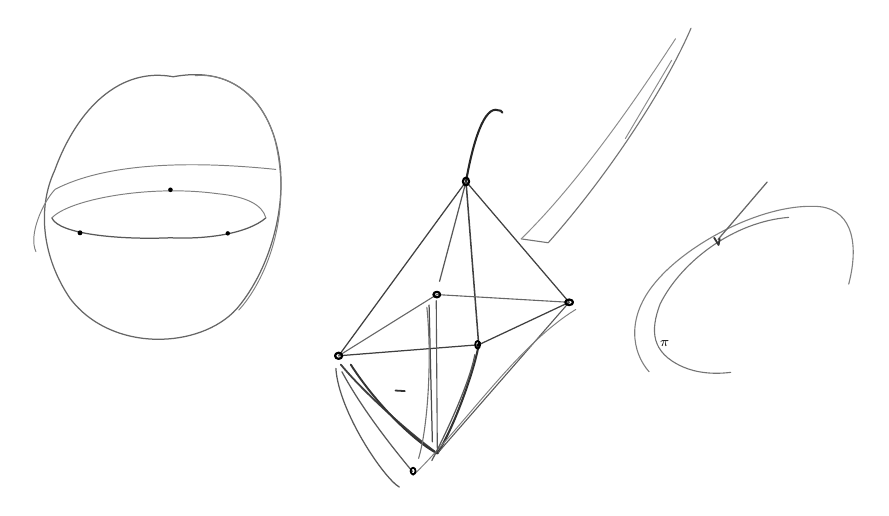
\begin{tikzpicture}[x=.007cm,y=-.007cm,line cap=round,line join=round]
\draw[black!60,line width=.45pt] (1550,418)
 .. controls (1454,400) and (1376,475) .. (1335,588)
 .. controls (1302,659) and (1314,748) .. (1363,820)
 .. controls (1438,919) and (1599,912) .. (1665,839)
 .. controls (1745,746) and (1780,566) .. (1701,465)
 .. controls (1664,422) and (1616,406) .. (1550,418);
\draw[black!50,line width=.35pt] (1590,416)
 .. controls (1664,410) and (1718,467) .. (1735,535)
 .. controls (1768,673) and (1715,791) .. (1669,841);
\draw[black!65,line width=.45pt] (1330,674)
 .. controls (1342,703) and (1450,714) .. (1545,710)
 .. controls (1610,713) and (1684,703) .. (1718,674);
\draw[black!50,line width=.35pt] (1330,674)
 .. controls (1360,641) and (1505,613) .. (1630,630)
 .. controls (1682,635) and (1712,650) .. (1718,674);
\draw[black!50,line width=.35pt] (1301,735)
 .. controls (1287,704) and (1314,645) .. (1336,622)
 .. controls (1425,576) and (1571,569) .. (1736,586);
\fill (1381,701) circle (4.5);
\fill (1649,702) circle (4);
\fill (1545,623) circle (4.2);
\coordinate (a) at (2081,608);
\coordinate (b) at (1850,924);
\coordinate (c) at (2104,904);
\coordinate (d) at (2268,827);
\coordinate (e) at (2028,813);
\coordinate (f) at (2029,1101);
\draw[black!75,line width=.45pt] (a)--(b)--(c)--(d)--(a);
\draw[black!75,line width=.55pt] (a)--(c);
\draw[black!60,line width=.4pt] (b)--(e)--(d);
\draw[black!65,line width=.45pt] (a)--(2033,789);
\draw[black!70,line width=.45pt] (2014,832)--(2020,1080);
\draw[black!65,line width=.4pt] (2027,824)--(f);
\draw[black!80,line width=.75pt] (c)
 .. controls (2096,951) and (2059,1055) .. (f);
\draw[black!65,line width=.4pt] (d)--(f);
\draw[black!75,line width=.65pt] (1854,940)
 .. controls (1897,992) and (1979,1065) .. (f);
\draw[black!80,line width=.7pt] (1872,940)
 .. controls (1921,1016) and (1991,1082) .. (f);
\draw[black!65,line width=.45pt] (1845,947)
 .. controls (1850,1025) and (1932,1146) .. (1960,1162);
\draw[black!65,line width=.45pt] (1856,953)
 .. controls (1892,1020) and (1948,1091) .. (1984,1134);
\draw[black!50,line width=.35pt] (1985,1141)
 .. controls (2078,1051) and (2174,905) .. (2280,840);
\draw[black!65,line width=.45pt] (2097,922)
 .. controls (2087,976) and (2040,1074) .. (2019,1114);
\draw[black!55,line width=.4pt] (2010,836)
 .. controls (2020,935) and (2011,1057) .. (1995,1110);
\draw[black!85,line width=.75pt] (a)
 .. controls (2093,539) and (2114,468) .. (2140,479)
 .. controls (2144,479) .. (2147,483);
\draw[black!55,line width=.4pt] (2181,712)--(2230,719)
 .. controls (2331,606) and (2439,446) .. (2489,330);
\draw[black!45,line width=.35pt] (2181,712)
 .. controls (2294,602) and (2408,430) .. (2461,349);
\draw[black!45,line width=.35pt] (2370,530)--(2454,388);
\draw[black!80,line width=.65pt] (1953,987)--(1970,988);
\draw[line width=.8pt] (2081,608) ellipse (5.5 and 7);
\draw[line width=.8pt] (1850,924) ellipse (6.5 and 5.5);
\draw[line width=.8pt] (2028,813) ellipse (6 and 5);
\draw[line width=.8pt] (2268,827) ellipse (7 and 5);
\draw[line width=.65pt] (2102,904) ellipse (4.5 and 7);
\fill (2103,900)--(2108,899)--(2105,905)--(2099,909)--cycle;
\draw[line width=.65pt] (1985,1133) ellipse (4.5 and 6);
\draw[black!50,line width=.4pt] (2775,794)
 .. controls (2796,713) and (2777,653) .. (2712,653)
 .. controls (2616,650) and (2484,720) .. (2426,789)
 .. controls (2370,854) and (2382,918) .. (2413,953);
\draw[black!55,line width=.4pt] (2666,673)
 .. controls (2567,681) and (2472,752) .. (2433,830)
 .. controls (2415,878) and (2416,918) .. (2474,944)
 .. controls (2499,955) and (2530,958) .. (2561,954);
\draw[black!60,line width=.45pt] (2538,713)--(2627,609);
\draw[black!80,line width=.65pt] (2531,710)--(2539,723)--(2541,712);
\node[font=\scriptsize,scale=.7,inner sep=0pt] at (2441,901) {$\unsure{\pi}$};
\end{tikzpicture}}

% The mechanical listing is upside down relative to the pencil sketches.
\figure{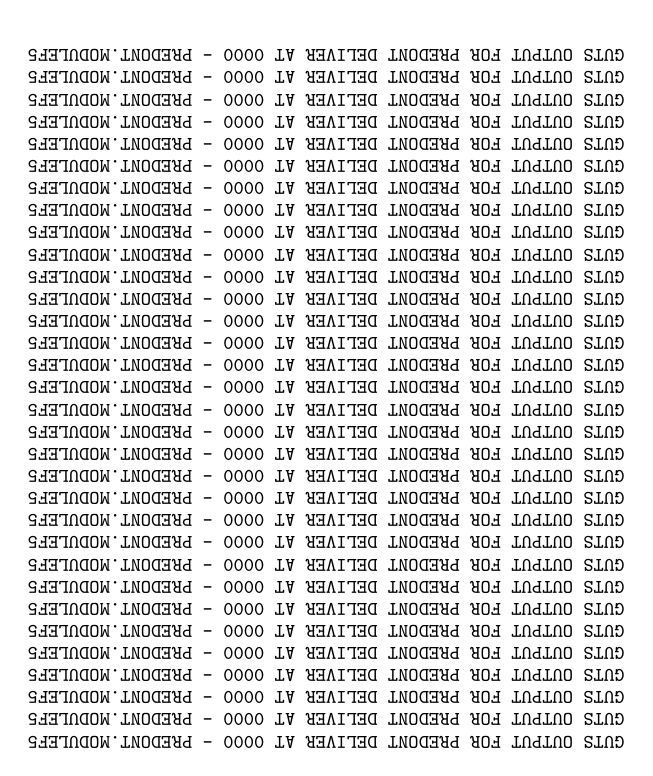
\begin{tikzpicture}
\node[rotate=180,align=left,font=\scriptsize,inner sep=0pt] {
\texttt{GUTS OUTPUT FOR PREDONT DELIVER AT 0000 - PREDONT.MODULEF5}\\
\texttt{GUTS OUTPUT FOR PREDONT DELIVER AT 0000 - PREDONT.MODULEF5}\\
\texttt{GUTS OUTPUT FOR PREDONT DELIVER AT 0000 - PREDONT.MODULEF5}\\
\texttt{GUTS OUTPUT FOR PREDONT DELIVER AT 0000 - PREDONT.MODULEF5}\\
\texttt{GUTS OUTPUT FOR PREDONT DELIVER AT 0000 - PREDONT.MODULEF5}\\
\texttt{GUTS OUTPUT FOR PREDONT DELIVER AT 0000 - PREDONT.MODULEF5}\\
\texttt{GUTS OUTPUT FOR PREDONT DELIVER AT 0000 - PREDONT.MODULEF5}\\
\texttt{GUTS OUTPUT FOR PREDONT DELIVER AT 0000 - PREDONT.MODULEF5}\\
\texttt{GUTS OUTPUT FOR PREDONT DELIVER AT 0000 - PREDONT.MODULEF5}\\
\texttt{GUTS OUTPUT FOR PREDONT DELIVER AT 0000 - PREDONT.MODULEF5}\\
\texttt{GUTS OUTPUT FOR PREDONT DELIVER AT 0000 - PREDONT.MODULEF5}\\
\texttt{GUTS OUTPUT FOR PREDONT DELIVER AT 0000 - PREDONT.MODULEF5}\\
\texttt{GUTS OUTPUT FOR PREDONT DELIVER AT 0000 - PREDONT.MODULEF5}\\
\texttt{GUTS OUTPUT FOR PREDONT DELIVER AT 0000 - PREDONT.MODULEF5}\\
\texttt{GUTS OUTPUT FOR PREDONT DELIVER AT 0000 - PREDONT.MODULEF5}\\
\texttt{GUTS OUTPUT FOR PREDONT DELIVER AT 0000 - PREDONT.MODULEF5}\\
\texttt{GUTS OUTPUT FOR PREDONT DELIVER AT 0000 - PREDONT.MODULEF5}\\
\texttt{GUTS OUTPUT FOR PREDONT DELIVER AT 0000 - PREDONT.MODULEF5}\\
\texttt{GUTS OUTPUT FOR PREDONT DELIVER AT 0000 - PREDONT.MODULEF5}\\
\texttt{GUTS OUTPUT FOR PREDONT DELIVER AT 0000 - PREDONT.MODULEF5}\\
\texttt{GUTS OUTPUT FOR PREDONT DELIVER AT 0000 - PREDONT.MODULEF5}\\
\texttt{GUTS OUTPUT FOR PREDONT DELIVER AT 0000 - PREDONT.MODULEF5}\\
\texttt{GUTS OUTPUT FOR PREDONT DELIVER AT 0000 - PREDONT.MODULEF5}\\
\texttt{GUTS OUTPUT FOR PREDONT DELIVER AT 0000 - PREDONT.MODULEF5}\\
\texttt{GUTS OUTPUT FOR PREDONT DELIVER AT 0000 - PREDONT.MODULEF5}\\
\texttt{GUTS OUTPUT FOR PREDONT DELIVER AT 0000 - PREDONT.MODULEF5}\\
\texttt{GUTS OUTPUT FOR PREDONT DELIVER AT 0000 - PREDONT.MODULEF5}\\
\texttt{GUTS OUTPUT FOR PREDONT DELIVER AT 0000 - PREDONT.MODULEF5}\\
\texttt{GUTS OUTPUT FOR PREDONT DELIVER AT 0000 - PREDONT.MODULEF5}\\
\texttt{GUTS OUTPUT FOR PREDONT DELIVER AT 0000 - PREDONT.MODULEF5}\\
\texttt{GUTS OUTPUT FOR PREDONT DELIVER AT 0000 - PREDONT.MODULEF5}\\
\texttt{GUTS OUTPUT FOR PREDONT DELIVER AT 0000 - PREDONT.MODULEF5}\\
};
\end{tikzpicture}}
\margin{31}

\scanpage{33}

\diagram{\[
\begin{array}{rll}
180 &
\left\{\begin{array}{l}
60=3\times20=2\times30\\
120=4\times30=2\times60
\end{array}\right. &
\begin{array}{l}f_{B,s}\\f_{\vec Q,a}\end{array}\\[1em]
420 &
\left\{\begin{array}{l}
60=1\times60=4\times60\\
\inserted{120=1\times120=1\times120}\\
60=1\times60=5\times12\\
60=1\times60=3\times20\\
120=1\times120=6\times20
\end{array}\right. &
\begin{array}{l}
\tau_{\pi,s}\\
\inserted{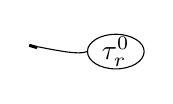
\begin{tikzpicture}[baseline=(z.base),x=1cm,y=1cm]
\node (z) at (.7,0) {$\tau_r^0$};
\draw (.7,0) ellipse (.36 and .22);
\draw (-.4,.08)..controls(-.1,.03)and(.2,-.05)..(.34,0);
\draw[line width=1.1pt](-.4,.08)--(-.3,.05);
\end{tikzpicture}}\\
\gamma_{\pi,s}\\
\gamma'_{\pi,s}\\
\gamma_r^0
\end{array}\\[1em]
\begin{array}{r}\inserted{1020}\\\deleted{\unsure{900}}\end{array} &
\left\{\begin{array}{l}
120=2\times60=1\times120\\
120=2\times60=2\times60\\
120=1\times120=2\times60\\
120=1\times120=2\times60\\
\inserted{3\times}120=\deleted{\unsure{2\times60=2\times60}}\inserted{3\times40=3\times40}\\
120=2\times60=2\times60\\
60=1\times60=2\times30
\end{array}\right. &
\begin{array}{l}
\tau_{\pi,\rho}\\
\gamma_{\pi,\rho}\\
\left.\begin{array}{l}
\unsure{\tau'_r|\tau_r^1}\\
\gamma_r^1\\
\gamma_r^{1'}\\
\gamma_r^2\\
\gamma_r^{2'}
\end{array}\right\}
\end{array}
\end{array}
\]}

\[
\begin{array}{r}
\overline{\overline{\deleted{\unsure{1580|1500}}}}\\
\inserted{1620}
\end{array}
=5\times60+\deleted{\unsure{12}}\inserted{11}\times120
\]

\[
\begin{array}{l}
\tau=\text{``twist''}\\
\gamma=\text{``gommage''}
\end{array}
\]

Programme de travail :

1) déterminer \unsure{les|un} syst. fondamental de
relations entre les \(1620\) flèches
du diagramme, se partageant
\deleted{entre} \(14\) \deleted{\unsure{paquets} de}\inserted{orbites} sous \(\unsure{\mathfrak S_K|\mathfrak G_K}\) (\unsure{aux|avec} \(542\)
sommets, se partageant entre \(9\) orbites)

\margin{en particulier, écrire toutes les flèches comme composés de flèches ``provenant de la dim. modulaire \(\leq1\)''}

\deleted{2) \unsure{Réduire}}

2) Reprendre la question, en éliminant
les sommets du niveau \(0\) (sauf
peut-être ceux de type \(\mathrm I_{10}\) ?),
\deleted{et \(\mathrm{II}_1\) (\unsure{qui} de type \(\mathrm{II}_1\) (qui \unsure{reviennent|revient}
à ceux de type \(\mathrm{III}_1\).) --- mais - Attention
au twist \inserted{\(\mathrm{tw}_{1/6}\)} \unsure{relationnel|relativement} : \(\mathrm{II}_1\) (qui donne
\unsure{un Autom.} de \(=\) type))}

3) Eliminer de plus les pièces
\deleted{\unsure{gauches}} ``tétraédrales'' \(\mathrm{II}_1\) --- et toutes
les pièces qui ne semblent pas
simplifier la présentation des relations.

\figure{\begin{tikzpicture}[x=.006cm,y=-.006cm,line cap=round,line join=round,
ink/.style={draw=black,line width=.6pt},
fine/.style={draw=black,line width=.35pt},
pencil/.style={draw=gray,line width=.35pt},
cut/.style={draw=green!40!black,line width=.8pt,dash pattern=on 1.2pt off 1.3pt},
cutsolid/.style={draw=green!40!black,line width=.8pt}]
% S033 pants
\draw[ink] (2343,133)..controls(2347,181)and(2338,216)..(2317,242);
\draw[ink] (2406,130)..controls(2413,177)and(2430,182)..(2480,180);
\draw[ink] (2482,232)..controls(2428,229)and(2400,244)..(2366,270);
\draw[ink] (2342,129)..controls(2336,117)and(2360,109)..(2380,113)..controls(2402,112)and(2415,118)..(2407,128)..controls(2390,141)and(2354,143)..cycle;
\draw[ink] (2317,242)..controls(2332,231)and(2344,237)..(2356,245)..controls(2370,254)and(2376,266)..(2366,273)..controls(2348,274)and(2328,261)..cycle;
\draw[ink] (2483,180)..controls(2497,176)and(2508,195)..(2504,215)..controls(2502,240)and(2483,243)..(2478,224)..controls(2472,208)and(2476,190)..cycle;
\draw[ink] (2341,239)..controls(2370,210)and(2391,174)..(2411,164)--(2418,170);
\draw[fine,dash pattern=on 1.1pt off 1.3pt] (2369,263)..controls(2397,241)and(2422,210)..(2438,181);
\draw[pencil] (2355,141)..controls(2350,178)and(2351,219)..(2342,240);
\draw[pencil] (2388,142)..controls(2420,172)and(2451,198)..(2481,202);
% S033 four_top
\draw[ink] (2649,129)..controls(2675,142)and(2702,145)..(2720,147);
\draw[ink] (2737,145)..controls(2752,142)and(2765,136)..(2766,131);
\draw[ink] (2798,152)..controls(2794,184)and(2794,213)..(2811,236);
\draw[ink] (2790,270)..controls(2768,233)and(2727,234)..(2684,283);
\draw[ink] (2634,260)..controls(2643,244)and(2649,234)..(2648,225);
\draw[ink] (2648,207)..controls(2652,191)and(2641,162)..(2632,153);
\draw[ink] (2616,149)..controls(2611,140)and(2636,118)..(2646,121)..controls(2660,124)and(2650,145)..(2624,155)..controls(2617,156)and(2615,154)..cycle;
\draw[ink] (2764,131)..controls(2773,115)and(2809,138)..(2807,149)..controls(2806,166)and(2774,152)..cycle;
\draw[ink] (2634,260)..controls(2649,251)and(2678,270)..(2683,284)..controls(2660,289)and(2633,278)..cycle;
\draw[ink] (2810,236)..controls(2819,246)and(2811,269)..(2799,275)..controls(2787,275)and(2786,265)..(2793,253)..controls(2799,243)and(2807,237)..cycle;
\draw[fine,dash pattern=on 1.2pt off 1.4pt] (2648,205)..controls(2699,188)and(2755,187)..(2797,200);
\draw[cut] (2648,205)..controls(2698,190)and(2756,191)..(2797,201);
\draw[fine,dash pattern=on 1.2pt off 1.4pt] (2725,147)..controls(2751,176)and(2741,215)..(2725,244);
\draw[cut] (2728,150)..controls(2752,182)and(2741,219)..(2729,243);
% S033 four_middle
\draw[ink] (2442,359)--(2390,448);
\draw[ink] (2487,361)..controls(2508,372)and(2534,376)..(2543,392)..controls(2546,414)and(2543,440)..(2540,456);
\draw[ink] (2410,468)..controls(2440,465)and(2496,466)..(2517,464);
\draw[ink] (2442,358)..controls(2449,343)and(2476,342)..(2487,356)..controls(2492,374)and(2447,380)..cycle;
\draw[ink] (2390,448)..controls(2397,442)and(2409,446)..(2413,457)..controls(2419,471)and(2408,475)..(2398,469)..controls(2389,463)and(2385,455)..cycle;
\draw[ink] (2521,445)..controls(2532,435)and(2543,444)..(2541,456)..controls(2540,468)and(2524,473)..(2518,460)..controls(2515,453)and(2518,449)..cycle;
\draw[ink] (2533,383)..controls(2544,386)and(2545,398)..(2535,403)..controls(2528,405)and(2526,397)..(2528,390)..cycle;
\draw[fine] (2450,367)--(2451,373) (2458,369)--(2459,374) (2467,369)--(2468,374);
\draw[ink] (2482,372)..controls(2496,395)and(2514,423)..(2530,442);
\draw[ink] (2394,458)--(2408,455);
\draw[fine,dash pattern=on 1.1pt off 1.4pt] (2414,451)..controls(2450,436)and(2492,422)..(2530,404);
\draw[fine,dash pattern=on 1.2pt off 1.3pt] (2408,408)..controls(2450,404)and(2480,409)..(2508,415);
\draw[cut] (2408,408)--(2447,464)--(2508,415)--cycle;
\draw[cut] (2508,415)--(2509,379)--(2543,420)--cycle;
% S033 cancelled_drawing
\draw[fine] (2669,407)--(2666,431);
\draw[ink] (2719,382)--(2730,394)..controls(2750,395)and(2783,407)..(2803,397);
\draw[pencil] (2796,399)..controls(2843,417)and(2838,440)..(2819,451);
\draw[ink] (2819,451)..controls(2804,463)and(2798,471)..(2807,487);
\draw[fine,dash pattern=on 1.3pt off 1.4pt] (2636,477)..controls(2673,449)and(2695,430)..(2750,441)..controls(2786,441)and(2792,455)..(2810,458);
\draw[fine,dash pattern=on 1.3pt off 1.4pt] (2655,499)..controls(2691,490)and(2710,488)..(2739,494);
\draw[fine] (2739,494)--(2787,503);
\draw[cut] (2764,402)..controls(2761,433)and(2750,469)..(2739,494);
\draw[cut] (2661,440)..controls(2714,427)and(2766,439)..(2810,458);
\draw[pencil,line width=.55pt] (2647,443)--(2748,383)--(2668,435)--(2778,385)--(2668,451)--(2787,397)--(2666,465)--(2776,423)--(2666,479)--(2791,430)--(2701,480)--(2802,450)--(2731,487)--(2794,471)--(2744,495)--(2790,483);
% S033 five_holes
\draw[ink] (2370,565)..controls(2356,599)and(2335,622)..(2296,632);
\draw[ink] (2450,570)..controls(2463,620)and(2485,642)..(2522,645);
\draw[ink] (2522,698)..controls(2487,725)and(2491,760)..(2493,787);
\draw[ink] (2458,812)..controls(2418,789)and(2386,799)..(2353,807);
\draw[ink] (2310,788)..controls(2315,736)and(2300,706)..(2276,683);
\draw[ink] (2370,565)..controls(2375,553)and(2437,551)..(2450,563)..controls(2458,579)and(2383,585)..cycle;
\draw[ink] (2296,632)..controls(2276,627)and(2265,666)..(2276,683)..controls(2295,681)and(2312,642)..cycle;
\draw[ink] (2522,645)..controls(2538,652)and(2540,692)..(2522,701)..controls(2510,697)and(2507,654)..cycle;
\draw[ink] (2310,788)..controls(2328,783)and(2360,798)..(2353,809)..controls(2338,822)and(2299,805)..cycle;
\draw[ink] (2493,787)..controls(2505,798)and(2494,813)..(2474,816)..controls(2457,819)and(2450,808)..(2464,798)..controls(2478,788)and(2487,785)..cycle;
\draw[cut] (2357,588)..controls(2394,631)and(2455,690)..(2507,706);
\draw[cut] (2317,621)..controls(2347,640)and(2355,676)..(2366,720);
\draw[cutsolid] (2366,720)..controls(2372,748)and(2393,775)..(2387,803);
\draw[cut] (2300,692)..controls(2340,659)and(2411,627)..(2460,604);
\draw[cut] (2478,642)..controls(2464,684)and(2449,707)..(2445,728);
\draw[cutsolid] (2443,736)..controls(2442,764)and(2437,781)..(2436,797);
\draw[cut] (2315,746)..controls(2336,738)and(2353,729)..(2363,726);
\draw[cutsolid] (2382,727)..controls(2403,727)and(2434,729)..(2443,736);
\draw[cut] (2454,738)..controls(2470,739)and(2478,744)..(2482,749);
\draw[pencil] (2296,632)..controls(2338,589)and(2362,558)..(2410,558)..controls(2470,561)and(2504,601)..(2516,646);
\draw[pencil] (2276,683)..controls(2276,748)and(2278,778)..(2310,788);
\draw[pencil] (2308,650)..controls(2380,638)and(2429,615)..(2460,604);
\draw[pencil] (2356,655)..controls(2411,641)and(2430,637)..(2478,642);
\draw[pencil] (2386,803)..controls(2410,781)and(2428,796)..(2463,811);
% S033 sphere_left
\draw[ink] (2259,980)..controls(2222,1010)and(2146,1022)..(2134,1117)..controls(2123,1190)and(2159,1226)..(2252,1249)..controls(2262,1253)and(2262,1264)..(2266,1268);
\draw[ink] (2338,982)..controls(2366,1015)and(2429,1017)..(2441,1093)..controls(2454,1194)and(2417,1230)..(2342,1251)..controls(2331,1260)and(2340,1267)..(2327,1270);
\draw[ink] (2259,977)..controls(2252,963)and(2329,960)..(2338,975)..controls(2343,988)and(2266,991)..cycle;
\draw[ink] (2266,1268)..controls(2284,1278)and(2314,1276)..(2327,1270);
\draw[fine,dash pattern=on 1.3pt off 1.3pt] (2267,1256)..controls(2279,1244)and(2318,1244)..(2332,1254);
\draw[ink] (2174,1141)..controls(2175,1113)and(2210,1110)..(2233,1140)..controls(2246,1168)and(2226,1191)..(2198,1183)..controls(2176,1179)and(2167,1162)..cycle;
\draw[ink] (2366,1146)..controls(2356,1120)and(2387,1102)..(2406,1115)..controls(2431,1133)and(2423,1166)..(2401,1174)..controls(2379,1182)and(2363,1171)..cycle;
\draw[fine,dash pattern=on 1.4pt off .7pt] (2261,1093)..controls(2262,1071)and(2288,1055)..(2309,1062)..controls(2328,1071)and(2338,1114)..(2319,1120)..controls(2297,1134)and(2261,1124)..cycle;
\draw[ink] (2132,1130)..controls(2143,1142)and(2160,1144)..(2172,1151);
\draw[ink] (2238,1157)..controls(2277,1166)and(2326,1162)..(2365,1152);
\draw[ink] (2423,1139)..controls(2432,1135)and(2437,1128)..(2442,1125);
\draw[fine,dash pattern=on .8pt off 1.1pt] (2135,1113)..controls(2176,1094)and(2219,1095)..(2261,1093);
\draw[fine,dash pattern=on 1.4pt off .8pt] (2330,1093)..controls(2369,1098)and(2405,1092)..(2442,1116);
\draw[pencil] (2250,992)..controls(2243,1048)and(2254,1115)..(2243,1173)..controls(2237,1216)and(2235,1230)..(2246,1248);
\draw[pencil] (2348,994)..controls(2357,1034)and(2328,1087)..(2340,1134)..controls(2346,1177)and(2370,1210)..(2351,1255);
\draw[pencil,line width=.5pt] (2155,1048)..controls(2190,1050)and(2232,1090)..(2267,1128)..controls(2306,1179)and(2335,1228)..(2351,1255);
\draw[pencil,dash pattern=on 1.1pt off 1.1pt] (2155,1048)..controls(2173,1101)and(2225,1155)..(2269,1202)..controls(2300,1230)and(2324,1243)..(2344,1255);
\draw[pencil,dash pattern=on 1pt off 1.1pt] (2245,1249)..controls(2273,1224)and(2302,1230)..(2346,1252);
\draw[pencil] (2243,1087)..controls(2240,1049)and(2317,1031)..(2400,1035)..controls(2444,1032)and(2442,1081)..(2422,1088);
\draw[pencil] (2330,1092)..controls(2365,1095)and(2401,1099)..(2422,1088);
\draw[pencil] (2357,1148)..controls(2351,1108)and(2395,1106)..(2426,1121)..controls(2449,1161)and(2426,1211)..(2387,1208)..controls(2355,1207)and(2348,1173)..cycle;
\draw[pencil] (2364,1145)..controls(2360,1118)and(2399,1114)..(2422,1131);
\draw[pencil] (2383,1126)..controls(2417,1127)and(2431,1148)..(2403,1143);
\draw[fine] (2132,1135)..controls(2129,1144)and(2133,1154)..(2127,1165)--(2134,1159);
% S033 sphere_right
\draw[ink] (2701,990)..controls(2686,1021)and(2595,1034)..(2564,1115)..controls(2547,1190)and(2590,1275)..(2668,1301)..controls(2730,1325)and(2854,1304)..(2880,1239)..controls(2916,1160)and(2913,1081)..(2878,1048)..controls(2854,1028)and(2816,1021)..(2810,997);
\draw[ink] (2701,986)..controls(2724,966)and(2785,976)..(2810,990)..controls(2825,1007)and(2736,1008)..cycle;
\draw[pencil] (2703,985)..controls(2735,980)and(2782,988)..(2805,999);
\draw[ink] (2619,1172)..controls(2611,1144)and(2642,1132)..(2664,1156)..controls(2688,1182)and(2660,1219)..(2635,1211)..controls(2622,1206)and(2616,1187)..cycle;
\draw[fine,line width=.6pt] (2813,1181)..controls(2817,1155)and(2841,1156)..(2856,1185)..controls(2872,1220)and(2846,1231)..(2825,1219)..controls(2812,1210)and(2810,1198)..cycle;
\draw[fine,dash pattern=on 1.3pt off .9pt] (2653,1105)..controls(2648,1084)and(2677,1075)..(2692,1092)..controls(2710,1115)and(2690,1146)..(2669,1138)..controls(2652,1133)and(2646,1120)..cycle;
\draw[fine,dash pattern=on 1.5pt off .6pt] (2824,1112)..controls(2816,1091)and(2842,1093)..(2860,1106)..controls(2882,1123)and(2867,1152)..(2844,1144)..controls(2826,1144)and(2820,1129)..cycle;
\draw[ink] (2564,1146)..controls(2572,1158)and(2598,1164)..(2618,1169);
\draw[ink] (2673,1190)..controls(2728,1190)and(2778,1202)..(2814,1198);
\draw[ink] (2860,1193)..controls(2880,1173)and(2887,1176)..(2898,1161);
\draw[fine,dash pattern=on 1.5pt off .9pt] (2568,1132)..controls(2597,1115)and(2629,1118)..(2651,1109);
\draw[fine] (2695,1104)..controls(2708,1110)and(2724,1111)..(2736,1111);
\draw[fine,dash pattern=on 1.4pt off 1pt] (2754,1111)..controls(2780,1115)and(2803,1117)..(2822,1112);
\draw[fine] (2870,1130)..controls(2884,1130)and(2895,1139)..(2900,1142);
\draw[pencil,line width=.65pt] (2669,1028)..controls(2629,1069)and(2597,1135)..(2596,1200)..controls(2599,1260)and(2635,1270)..(2670,1234)..controls(2728,1170)and(2775,1073)..(2809,1020);
\draw[pencil,line width=.6pt] (2812,1022)..controls(2778,1093)and(2744,1163)..(2675,1237);
\draw[pencil] (2671,1026)..controls(2663,1079)and(2661,1154)..(2674,1237)..controls(2684,1277)and(2701,1300)..(2714,1308);
\draw[pencil,dash pattern=on 1.4pt off 1.1pt] (2673,1024)..controls(2722,1037)and(2723,1104)..(2729,1176)..controls(2730,1257)and(2725,1289)..(2714,1308);
\draw[pencil,line width=.5pt] (2816,1021)..controls(2808,1072)and(2785,1142)..(2770,1214)..controls(2764,1263)and(2751,1301)..(2758,1309);
\draw[pencil,dash pattern=on 1.4pt off 1.2pt] (2820,1027)..controls(2830,1092)and(2809,1170)..(2795,1243)..controls(2784,1285)and(2769,1302)..(2758,1309);
\draw[fine,line width=.65pt] (2745,1310)--(2715,1310)--(2737,1320);
\draw[fine,line width=.65pt] (2783,1304)--(2808,1296)--(2796,1308);
% S033 isolated_arc
\draw[pencil] (1978,699)..controls(1976,753)and(2037,766)..(2056,724);
% S033 grouping
\draw[pencil] (2309,139)..controls(2279,178)and(2264,271)..(2304,298)..controls(2379,315)and(2497,283)..(2561,210)..controls(2612,157)and(2605,118)..(2615,82);
\draw[pencil] (2615,82)..controls(2653,40)and(2674,27)..(2710,18);
\draw[pencil] (2770,20)..controls(2843,58)and(2926,134)..(2898,217)..controls(2862,326)and(2767,392)..(2647,455)..controls(2538,514)and(2416,540)..(2361,498)..controls(2321,465)and(2319,403)..(2352,365);
\draw[pencil] (2154,854)..controls(2205,703)and(2244,570)..(2322,532)..controls(2408,498)and(2569,512)..(2642,564)..controls(2701,608)and(2713,758)..(2768,808)..controls(2855,871)and(2915,1014)..(2919,1161)..controls(2916,1312)and(2909,1375)..(2812,1379)..controls(2669,1376)and(2556,1364)..(2456,1374)..controls(2303,1385)and(2133,1356)..(2084,1306)..controls(2029,1247)and(2048,1086)..(2079,977)..controls(2098,920)and(2135,897)..(2154,854);
\draw[pencil] (1950,1406)..controls(1978,1421)and(2014,1410)..(2059,1414)--(2855,1418);
% S033 large_surface
\draw[pencil] (2048,1682)..controls(1996,1624)and(2047,1571)..(2168,1504)..controls(2211,1479)and(2250,1473)..(2276,1491)..controls(2314,1540)and(2249,1631)..(2168,1672)..controls(2109,1701)and(2055,1707)..(2048,1682);
\draw[fine,line width=.55pt] (2276,1491)..controls(2302,1534)and(2264,1597)..(2227,1635)..controls(2178,1673)and(2098,1709)..(2048,1682);
\draw[pencil] (2044,1685)..controls(2124,1717)and(2246,1660)..(2288,1570)..controls(2305,1530)and(2292,1504)..(2276,1491);
\foreach \x/\y in {2276/1491,2257/1600,2168/1672,2048/1682,2069/1585,2168/1504}{
\draw[fine,line width=.7pt] (\x-8,\y)--(\x+8,\y) (\x-5,\y-7)--(\x+5,\y+7) (\x-5,\y+7)--(\x+5,\y-7);
}
\foreach \x/\y in {2285/1549,2227/1635,2110/1690,2048/1627,2110/1543,2218/1485}{\fill (\x,\y) circle[radius=.7pt];}
\draw[fine,line width=.6pt] (2284,1517)--(2296,1512)
(2261,1573)--(2289,1584)
(2241,1613)--(2249,1618)
(2196,1648)--(2204,1655)
(2137,1671)--(2148,1694)
(2080,1688)--(2080,1697)
(2035,1652)--(2043,1652)
(2047,1603)--(2069,1612)
(2085,1561)--(2094,1567)
(2132,1522)--(2138,1528)
(2185,1487)--(2193,1504)
(2246,1478)--(2246,1486);
\draw[fine] (2048,1682)..controls(2091,1781)and(2164,1879)..(2154,1982)..controls(2156,2084)and(2068,2184)..(2019,2219);
\draw[pencil] (2048,1682)..controls(2108,1802)and(2182,1889)..(2174,1987)..controls(2156,2064)and(2076,2111)..(2003,2154);
\draw[pencil] (2048,1682)..controls(2070,1734)and(2090,1752)..(2115,1775);
\draw[fine] (2276,1491)..controls(2340,1613)and(2472,1700)..(2575,1745)..controls(2701,1793)and(2855,1734)..(2968,1721)..controls(2980,1717)and(2989,1723)..(2995,1731);
\draw[pencil] (2281,1505)..controls(2334,1620)and(2499,1704)..(2583,1741)..controls(2719,1773)and(2856,1724)..(2963,1719);
\draw[pencil] (2291,1518)..controls(2338,1582)and(2401,1634)..(2489,1677);
\draw[pencil] (2973,1727)..controls(2940,1802)and(2924,1949)..(2936,2026)..controls(2939,2050)and(2952,2057)..(2962,2064);
\draw[fine] (2962,1734)..controls(2930,1812)and(2920,1944)..(2927,2017)..controls(2931,2043)and(2950,2060)..(2961,2066);
\draw[pencil] (2980,1733)..controls(2963,1805)and(2964,1899)..(2970,1938);
\draw[pencil] (2955,2071)..controls(2823,2099)and(2721,2150)..(2630,2217);
\draw[pencil] (2949,2066)..controls(2818,2097)and(2688,2160)..(2625,2228);
\draw[pencil] (2940,2051)..controls(2897,2050)and(2847,2083)..(2821,2102);
\draw[pencil] (2019,2219)..controls(2015,2201)and(2058,2209)..(2080,2228);
\end{tikzpicture}}

\margin{32}

\scanpage{34}
\mspage{1}
Systèmes spéciaux de cinq points sur une sphère complexe (plus gén.\textsuperscript{t} sur une \deleted{\unsure{courbe}} droite projective sur un corps alg clos \(k\) \unsure{de car. \(0\)})

Ce sont les systèmes \((\Sigma,K)\) avec \(K\subset\Sigma\), \(\operatorname{card}K=5\), et tels qu’il existe un autom. non trivial de \((\Sigma,K)\) --- i.e. le groupe \inserted{\(G\)} des automorphismes de \((\Sigma,K)\) n’est pas réduit à \(1\). On fait la classification suivant la structure de ce groupe.

Soit \(g\in G\) d’ordre maximal. On peut identifier \(g\) à une permutation de \(I\), et la discussion se fait suivant la structure de celle-ci. Notons que \deleted{l’ordre de \(g\ne1\) est} tout autom. d’ordre fini de \(\Sigma\) \deleted{\(\unsure{\nu}\,g\) d’ordre \(5\)} a exactement deux pts fixes, et que \deleted{\unsure{il est}} \inserted{si l’ordre est \(\nu\)}, \(\mathbb Z/\nu\mathbb Z\) opère librement sur \(\Sigma\setminus\Sigma^g\). Cela montre que
\[
K=K^g\amalg\text{orbites d’ordre }\nu,\quad\text{donc }2\leq\nu\leq5.
\]
\margin{l’opération est celle de \(\mu_\nu\) sur \(\widehat{\mathbb G}_m\)}

\textcircled{1} \(\nu=5\), alors \(K\) est une orbite --- OPS que c’est l’orbite \(\mu_5(k)\) de \(\mu_5\) opérant sur \(\mathbb P^1_k\). Le groupe total des autom. est \tikz[baseline=(d.base)]{\node[draw,circle,inner sep=1pt] (d) {\(\mathbb D_5\)};}. À isom. près, il y a un seul tel cas.

\margin{Structure pentagonale sur \(I\) (``pentagone'')}
\figure{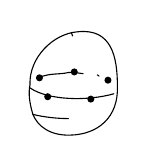
\begin{tikzpicture}[scale=.75,line cap=round,line join=round]
\draw (-.73,-.03) .. controls (-.75,.43) and (-.34,.84) .. (.08,.87)
 .. controls (.65,.93) and (.75,.45) .. (.75,-.05)
 .. controls (.77,-.58) and (.42,-.87) .. (-.05,-.88)
 .. controls (-.39,-.89) and (-.60,-.73) .. (-.68,-.53)
 .. controls (-.74,-.34) and (-.76,-.16) .. (-.73,-.03);
\draw (-.73,-.08) .. controls (-.43,-.29) and (.23,-.31) .. (.69,-.18);
\draw (-.60,.09) .. controls (-.36,.18) and (-.25,.14) .. (-.08,.18)
 .. controls (.01,.19) and (.09,.17) .. (.17,.16);
\draw (.41,.14)--(.44,.12);
\draw (.59,.07)--(.61,.02);
\foreach \x/\y in {-.57/.09,.02/.19,.59/.05,-.43/-.23,.30/-.27}
 {\fill (\x,\y) circle(1.7pt);}
\draw (-.68,-.53) .. controls (-.47,-.58) and (-.25,-.60) .. (-.08,-.60);
\draw (-.03,.86)--(-.01,.80);
\end{tikzpicture}}

\textcircled{2} \(\nu=4\) alors \deleted{\(\unsure{K|\Sigma}=\operatorname{card}I^g=1\)} \inserted{\(K^g=\{P\}\)}, et \(I\setminus\{P\}\) est une orbite. OPS que c’est \(\mu_4\), sur lequel \(\mu_4\) opère, et \(P\) est un pôle : \(\unsure{\infty}\). Le groupe total des autom. est \(\mathbb Z/4\mathbb Z\simeq\mu_4(k)\).

La catégorie de ces configurations est équivalente à celle des carrés orientés.

\margin{``pyramide carrée''}
\figure{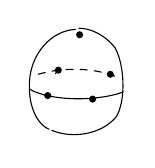
\begin{tikzpicture}[scale=.75,line cap=round,line join=round]
\draw (-.02,.89) .. controls (-.43,.87) and (-.78,.48) .. (-.80,-.01)
 .. controls (-.82,-.49) and (-.62,-.74) .. (-.47,-.80);
\draw (-.42,-.82) .. controls (-.05,-.97) and (.43,-.88) .. (.67,-.59)
 .. controls (.84,-.31) and (.81,.29) .. (.65,.58)
 .. controls (.45,.83) and (.20,.91) .. (.04,.91);
\draw (-.80,-.12) .. controls (-.44,-.33) and (.35,-.33) .. (.79,-.17);
\draw[dash pattern=on 2.6pt off 2.5pt] (-.65,.13)
 .. controls (-.25,.25) and (.30,.25) .. (.69,.08);
\foreach \x/\y in {.05/.80,-.49/-.23,.27/-.29,-.31/.20,.57/.13}
 {\fill (\x,\y) circle(1.7pt);}
\draw (-.31,.20)--(-.36,.14);
\end{tikzpicture}}

\textcircled{3} \(\nu=3\), Alors \deleted{\(\unsure{\Sigma|K}\)} \(\operatorname{card}K^g=2\), \inserted{donc \(K^g=\Sigma^g\)}, et \(I\setminus K^g\) \inserted{\(=J\)} est une orbite,
\deleted{Le groupe total est}
\inserted{qu’on peut supposer \(\mu_3\).} La catégorie de ces configurations est équivalente : celle des triangles combinatoires i.e. celle \(\mathrm{Ens}(3)\) des ens \(J\) de card \(3\).

A \(J\) on associe \(\Sigma_J\deleted{\unsure{\Sigma}}\) avec \(J\cup P_J\) (\(P_J\subset\Sigma_J^{\unsure{g}}\) ens des deux pôles de \(\Sigma_J\) pour corr. \(1\)-\(1\) avec l’ens \(\omega(I)\) des or. de \(J\), si \(\unsure{k|K}=\mathbb C\)). Groupe des autom. est \(\mathbb D_3\).

\margin{\unsure{Partition} \(2\) et \(3\) (par ordre de \unsure{cardinaux|valeurs} ou symétries)}
\margin{``bitétraèdre''}
\figure{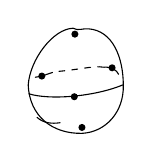
\begin{tikzpicture}[scale=.75,line cap=round,line join=round]
\draw (-.80,-.08) .. controls (-.77,.35) and (-.38,.87) .. (-.04,.88)
 .. controls (.04,.83) and (.13,.88) .. (.22,.87)
 .. controls (.63,.84) and (.81,.39) .. (.81,-.09)
 .. controls (.82,-.53) and (.52,-.88) .. (.11,-.90)
 .. controls (-.39,-.91) and (-.78,-.61) .. (-.80,-.08);
\draw (-.79,-.23) .. controls (-.44,-.34) and (.32,-.28) .. (.80,-.08);
\draw (-.68,.05) .. controls (-.56,.06) and (-.47,.11) .. (-.39,.13);
\draw[dash pattern=on 2.1pt off 2.6pt] (-.28,.15)
 .. controls (.06,.18) and (.33,.25) .. (.47,.22);
\draw (.48,.22) .. controls (.61,.23) and (.70,.17) .. (.73,.10);
\foreach \x/\y in {-.01/.78,.11/-.80,-.02/-.28,-.57/.07,.62/.21}
 {\fill (\x,\y) circle(1.7pt);}
\draw (-.65,-.63) .. controls (-.54,-.73) and (-.40,-.74) .. (-.26,-.72);
\end{tikzpicture}}
\margin{33}

\scanpage{35}
\mspage{2}
\textcircled{4} \(\nu=2\). \deleted{Il y a \unsure{deux cas}} \inserted{\unsure{Dans ce cas}} \(K^g=\{P\}\), et \(K\setminus K^g\) \inserted{\(=I\)} est réunion de deux orbites. Ainsi, \(g\) est un autom. \deleted{\unsure{de}} ``universel'' de \(\Sigma\setminus I\) (\(g\in V(\unsure{D_I|\mathbb D_I})\)) et \(P\) est \inserted{\unsure{un de|un}} \deleted{\unsure{un}} p\textsuperscript{t} fixe. \deleted{\unsure{De}} Cette fois, la situation a des ``modules'', p.ex. en choisissant une des deux orbites,

\deleted{\unsure{OPS} que l’opération de \(g\) sur elle est celle de \(\mu_2\) \inserted{\(=\{\pm1\}\)} sur \(\mu_2\) \inserted{\(=\{\pm1\}\)}, et \(P=0\), l’autre orbite est \deleted{\unsure{donnée par}} un \(\{t,-t\}\), avec \(\lambda=t^2\ne1,\lambda\in k^\times\) ---
donc \deleted{\(\lambda=\)} \(J=(0,\pm1,\pm\sqrt\lambda)\) \deleted{\(\unsure{\sqrt\lambda,\sqrt\lambda}\)}, avec \(\lambda\in\Sigma(k)\setminus\{0,1,\infty\}\),
\unsure{en} \deleted{\unsure{changeant}} changeant le choix de l’orbite, on trouve
\[
(0,\pm1,\pm\sqrt{1/\lambda}).
\]
Prenons le paramètre \(\rho=\lambda+\frac1\lambda\), \inserted{\(\ne2\)}, donc \(\lambda^2-\rho\lambda+1=0\),
\deleted{\(\lambda=\frac12(\rho\pm\sqrt{\rho^2-4})\)},
on trouve \((0,\pm1,\pm\sqrt{\frac12(\rho\pm\sqrt{\rho^2-4})})\).
\unsure{Comme} \(0,\infty\), et \unsure{deux} \unsure{discriminant différent} \(2,\infty\) --- \unsure{comme} \deleted{\unsure{les}} \(\lambda\), et
\(g(z)=\frac{\lambda}{z}\), p\textsuperscript{ts} fixes}

Cas moins intéressant que les précédents, \unsure{du|de} notre point de vue, car il y a des modules. Quand la structure \((\Sigma,I)\) est une structure carrée, on retrouve soit le cas \(2^\circ\) (si \(g\) laisse stables les deux diagonales), soit le cas \inserted{des sommets} d’un \deleted{\unsure{carré|cas}} carré sphérique \unsure{équilatéral}\unsure{,} et du milieu de l’une des arêtes. \inserted{Est-ce le cas \(1^\circ\) ?} Quand c’est une structure tétraédrale, \(P\) est un des \inserted{\(6\)} sommets de l’octaèdre associé.

\figure{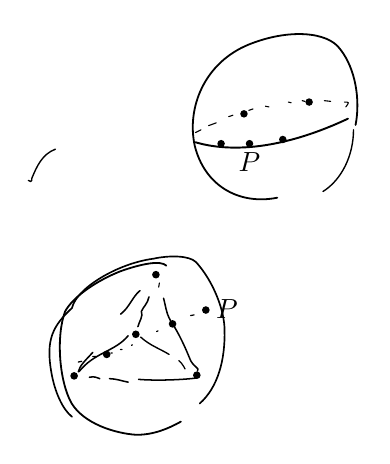
\begin{tikzpicture}[x=.0088cm,y=-.0088cm,line cap=round,line join=round]
% Upper sphere: the contour is open at lower right and has a short right-side gap.
\draw[line width=.65pt] (383,249)
 .. controls (327,260) and (278,231) .. (264,174)
 .. controls (252,119) and (278,54) .. (342,28)
 .. controls (399,5) and (456,9) .. (474,35)
 .. controls (496,63) and (503,108) .. (496,144);
\draw[line width=.5pt] (493,151)
 .. controls (493,188) and (476,223) .. (449,240);
\draw[line width=.7pt] (265,169)
 .. controls (323,186) and (400,175) .. (485,135);
% Rear equatorial arc, with the irregular short dashes visible on the sheet.
\draw[line width=.4pt] (265,155)--(273,151)
 (284,145)--(295,141) (313,132)--(319,130)
 (342,123)--(348,121) (366,117)--(371,118)
 (399,111)--(403,112) (419,109)--(423,110)
 (451,109)--(460,110) (480,111)..controls(487,111)..(482,118);
\foreach \x/\y in {302/171,343/171,391/165,335/128,429/111}
 {\fill (\x,\y) circle[radius=5.4];}
\node[below,inner sep=1pt] at (343,179) {$P$};
% Detached curved stroke at the left, without a supplied arrowhead.
\draw[line width=.5pt] (63,179)..controls(44,186)and(36,204)..(29,221)
 ..controls(30,227)and(25,226)..(24,224);
\begin{scope}[shift={(25,305)}]
% Lower sphere: the two left-hand contours and the open lower-right contour.
\draw[line width=.65pt] (198,42)
 ..controls(190,34)and(163,39)..(132,50)
 ..controls(99,63)and(64,86)..(52,108)
 ..controls(39,143)and(43,207)..(61,240)
 ..controls(79,270)and(124,284)..(155,286)
 ..controls(180,286)and(201,277)..(219,267);
\draw[line width=.6pt] (62,103)
 ..controls(34,129)and(24,149)..(32,195)
 ..controls(37,225)and(49,250)..(62,260);
\draw[line width=.6pt] (62,103)
 ..controls(68,75)and(127,39)..(179,32)
 ..controls(202,27)and(231,27)..(241,37)
 ..controls(267,66)and(282,108)..(282,135)
 ..controls(283,179)and(272,218)..(246,241);
% Broken outer triangular sides and rear branches, preserving their gaps.
\draw[line width=.55pt] (160,78)..controls(149,87)and(145,102)..(132,112);
\draw[line width=.55pt] (92,167)..controls(82,178)and(73,186)..(71,195);
\draw[line width=.55pt] (194,89)..controls(198,104)and(198,113)..(207,126)
 ..controls(216,140)and(224,157)..(231,174)
 ..controls(236,189)and(247,189)..(243,194);
\draw[line width=.55pt] (87,203)..controls(94,201)and(99,204)..(102,205)
 (116,205)..controls(126,205)and(136,209)..(143,210)
 (158,206)..controls(180,208)and(219,207)..(242,204);
\draw[line width=.55pt] (173,87)..controls(171,97)and(165,101)..(162,108)
 ..controls(165,115)and(159,122)..(157,130);
\draw[line width=.55pt] (143,143)..controls(124,166)and(94,167)..(72,195);
\draw[line width=.5pt] (161,145)..controls(174,157)and(189,162)..(202,170);
\draw[line width=.45pt] (216,179)..controls(220,182)and(223,187)..(225,191);
% Dotted oblique slant, including the short dash next to P.
\draw[line width=.45pt] (71,181)--(76,180) (92,173)--(97,173)
 (118,168)--(120,168) (132,163)--(134,163)
 (148,157)--(149,156) (184,137)--(186,136)
 (233,114)--(238,113);
\draw[line width=.4pt] (188,67)--(187,73);
\foreach \x/\y in {183/55,65/201,242/200,154/141,112/170,207/126,255/106}
 {\fill (\x,\y) circle[radius=5.5];}
\node[right,inner sep=2pt] at (261,105) {$P$};
\end{scope}
\end{tikzpicture}}

\uline{Cas des antiautomorphismes \inserted{\(\sigma\)} de} \(\Sigma\) laissant \uline{stables} \(K\). \inserted{\unsure{(}Cas \(k=\mathbb C\))} Comme \unsure{il|\(\sigma\)} est d’ordre pair, on voit qu’il \deleted{\unsure{a}} a un p\textsuperscript{t} fixe au moins dans \(K\), donc dans \(\Sigma\), et étant d’ordre fini, on voit qu’il est d’ordre \(2\), il correspond à une structure réelle sur \(\Sigma\), \deleted{\unsure{et}}
On distingue suivant le cardinal de \(K^\sigma\), qui est \(1,3\), ou \(5\).
\margin{34}

\scanpage{36}
\mspage{3}

a) \(K^\sigma=K\) --- on trouve ess.\textsuperscript{t} les points réels de
\(M_{0,5}^{!}\simeq\mathrm{Sym}_2^*(U_{0,3})\),
\deleted{\unsure{Le cas|un cas}} de dim réelle \(2\) : contient le cas \(1^\circ\) (pentagonal)

b) \(\operatorname{card}K^\sigma=3\). En prenant pour repère \(0,1,\infty\) dans \(K^\sigma\), on trouve que
\[
K=\{0,1,\infty,\lambda,\bar\lambda\},\quad
\lambda\in\text{demi-plan de Poincaré},\quad\text{dim réelle }2.
\]
Contient le cas \(3^\circ\) (bitétraédral)
\margin{OPS \(\sigma z=\bar z\) \deleted{\unsure{pour} \(\sigma z=\bar z\)}}

c) \(\operatorname{Card}K^\sigma=1\), i.e. \deleted{\unsure{?}} \(K^\sigma=\{P\}\),
\inserted{\unsure{Soit} \(K\setminus K^\sigma=I\),}
\deleted{on prend \unsure{comme repère} \(\infty\), et on choisit un p\textsuperscript{t} \(0\) tel que \(0=\sigma0\). OP}

\((\Sigma,I)\) est un syst. de \(4\) pts sur une sphère complexe,
\deleted{muni d’} \inserted{\unsure{admettant}} un antiautomorphisme
\deleted{\(\unsure{\sigma}\)} involutif (``conjugaison''), ils sont bien connus et de dim
modulaire \uline{réelle} \(1\), de plus le choix d’un p\textsuperscript{t}
réel supplémentaire \(P\) fait une dim. de
plus, soit dim réelle totale \(2\) encore.
(Contient le cas pyramidal carré, \(2^\circ\))

\figure{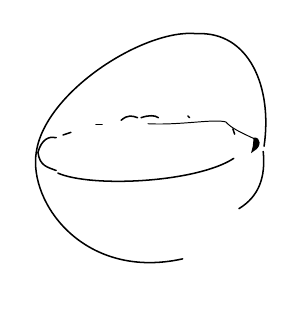
\begin{tikzpicture}[x=.011cm,y=-.011cm,line width=.55pt,line cap=round,line join=round]
\draw (289,1180) .. controls (176,1205) and (111,1116) .. (120,1057)
 .. controls (130,987) and (245,914) .. (305,920)
 .. controls (366,917) and (393,982) .. (383,1050);
\draw (382,1056) .. controls (385,1086) and (377,1108) .. (354,1122);
\draw (122,1057) .. controls (126,1042) and (135,1038) .. (143,1040);
\draw (151,1037)--(160,1034);
\draw (189,1025)--(196,1025);
\draw (218,1020) .. controls (226,1013) and (231,1015) .. (237,1017);
\draw (241,1017) .. controls (250,1014) and (257,1014) .. (261,1017);
\draw (295,1015)--(297,1017);
\draw[line width=.35pt] (249,1024) .. controls (286,1026) and (326,1018) .. (339,1022)
 .. controls (345,1029) and (356,1034) .. (371,1041);
\draw (347,1030)--(349,1036);
\draw (122,1057) .. controls (124,1073) and (133,1074) .. (143,1078);
\draw (145,1081) .. controls (184,1098) and (305,1092) .. (348,1064);
\fill (371,1040) .. controls (380,1039) and (380,1051) .. (372,1055)
 --(368,1058)--(370,1050)--cycle;
\end{tikzpicture}}

\figure{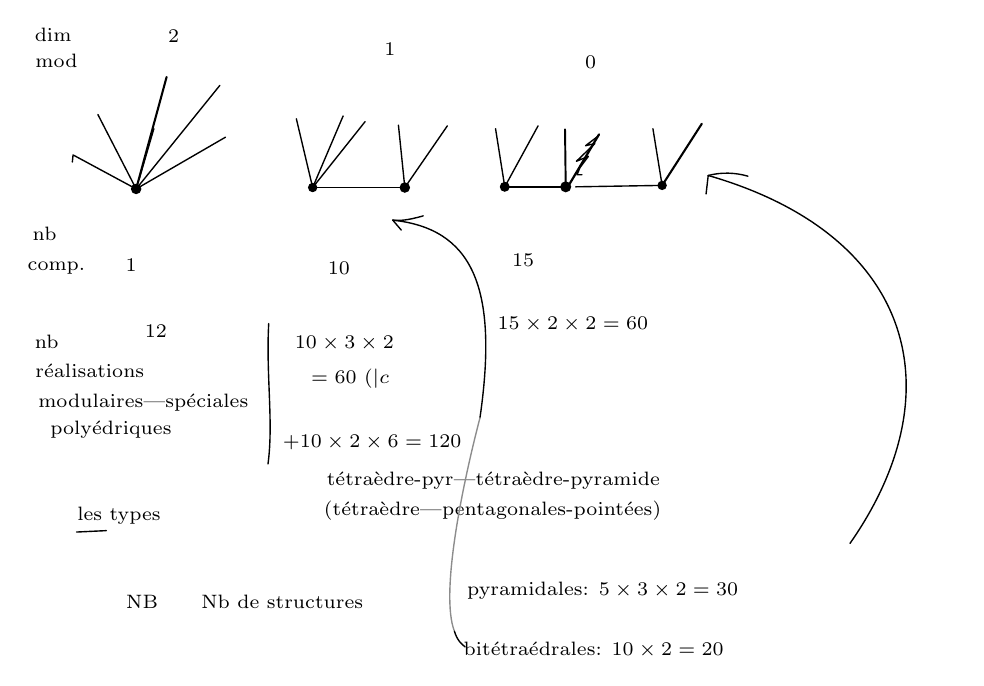
\begin{tikzpicture}[x=.009cm,y=-.009cm,line width=.5pt,line cap=round,line join=round,font=\scriptsize,inner sep=0pt]
\node[anchor=west] at (30,1535) {dim};
\node[anchor=west] at (31,1572) {mod};
\node at (227,1538) {$2$};
\node at (532,1556) {$1$};
\node at (815,1575) {$0$};
% Five free branches at a single vertex.
\draw (174,1753)--(85,1705)--(84,1715);
\draw (174,1753)--(120,1648);
\draw[line width=.75pt] (174,1753)--(217,1595);
\draw (178,1740)--(199,1668);
\draw (174,1753)--(292,1607);
\draw (174,1753)--(300,1680);
\fill (174,1753) circle (1.9pt);
% Two joined vertices and their three plus two branches.
\draw (423,1751)--(553,1751);
\draw (423,1751)--(400,1654);
\draw (423,1751)--(466,1650);
\draw (423,1751)--(497,1658);
\draw (553,1751)--(544,1663);
\draw (553,1751)--(613,1664);
\fill (423,1751) circle (1.7pt);
\fill (553,1751) circle (1.9pt);
% The sloping extra middle branch is crossed out; the upright remains.
\draw (694,1750)--(780,1750);
\draw (794,1750)--(916,1748);
\draw (694,1750)--(681,1668);
\draw (694,1750)--(741,1664);
\draw[line width=.7pt] (780,1750)--(779,1669);
\draw[line width=.8pt] (783,1750)--(827,1676);
\draw (825,1679)--(808,1692)--(821,1689)--(795,1714)--(812,1707)
 --(800,1723)--(796,1733)--(803,1733);
\draw (916,1748)--(903,1668);
\draw[line width=.75pt] (916,1748)--(972,1661);
\fill (694,1750) circle (1.8pt);
\fill (780,1750) circle (2pt);
\fill (916,1748) circle (1.7pt);
\node[anchor=west] at (27,1816) {nb};
\node[anchor=west] at (20,1865) {comp.};
\node at (167,1860) {$1$};
\node at (460,1865) {$10$};
\node at (720,1854) {$15$};
\node at (202,1954) {$12$};
\node[anchor=west] at (30,1968) {nb};
\node[anchor=west] at (31,2010) {réalisations};
\node[anchor=west] at (35,2054) {\unsure{modulaires|spéciales}};
\node[anchor=west] at (52,2092) {\deleted{\unsure{polyédriques}}};
\draw (361,1943) .. controls (357,2015) and (368,2082) .. (360,2141);
\node[anchor=west] at (397,1971) {$10\times3\times2$};
\node[anchor=west] at (420,2020) {$=60\ \unsure{(|c}$};
\node[anchor=west] at (380,2110) {$+10\times2\times6=120$};
\node[anchor=west] at (683,1944) {$15\times2\times2=60$};
\node[anchor=west] at (442,2164) {\deleted{\unsure{tétraèdre-pyr|tétraèdre-pyramide}}};
\node[anchor=west] at (438,2207) {(\unsure{tétraèdre|pentagonales}-pointées)};
\node[anchor=west] at (90,2214) {\deleted{\unsure{les types}}};
\draw (90,2237)--(132,2235);
\node[anchor=west] at (159,2335) {\uline{NB}};
\node[anchor=west] at (265,2335) {Nb de structures};
\node[anchor=west] at (640,2320) {pyramidales: $5\times3\times2=30$};
\node[anchor=west] at (635,2404) {bitétraédrales: $10\times2=20$};
% Arrows from the two structure counts to the corresponding graphs.
\draw (1181,2253) .. controls (1330,2040) and (1272,1818) .. (981,1734);
\draw (981,1734)--(978,1760);
\draw (981,1734) .. controls (1000,1729) and (1020,1730) .. (1037,1735);
\draw (536,1797) .. controls (647,1809) and (686,1889) .. (659,2076);
\draw[black!45] (659,2076) .. controls (636,2164) and (602,2323) .. (623,2377);
\draw (623,2377) .. controls (627,2390) and (633,2395) .. (638,2399);
\draw (536,1797)--(548,1811);
\draw (536,1797) .. controls (550,1799) and (568,1794) .. (579,1791);
\end{tikzpicture}}

\figure{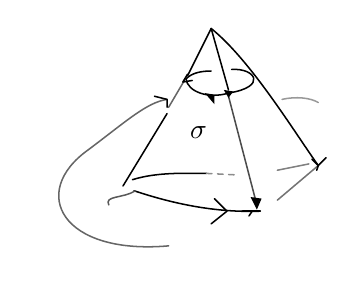
\begin{tikzpicture}[x=.02cm,y=-.02cm,line width=.55pt,line cap=round,line join=round]
\draw (1235,2700)--(1220,2730);
\draw[black!60] (1218,2733)--(1208,2750);
\draw (1207,2754)--(1179,2800);
\draw (1235,2700) .. controls (1260,2720) and (1288,2766) .. (1303,2787);
\draw (1235,2700)--(1246,2739);
\draw[black!70] (1246,2743)--(1264,2812);
\fill (1260,2807)--(1264,2815)--(1267,2808)--cycle;
\draw (1185,2796) .. controls (1201,2791) and (1219,2792) .. (1232,2792);
\draw[black!45,dash pattern=on 2pt off 2pt] (1232,2792)--(1252,2793);
\draw[black!50] (1277,2790)--(1297,2786);
\draw[black!55] (1277,2809)--(1303,2787);
\draw (1303,2787)--(1308,2782);
\draw (1299,2783)--(1303,2787)--(1302,2790);
\draw (1186,2803) .. controls (1210,2811) and (1237,2817) .. (1266,2816);
\draw (1237,2808)--(1245,2816)--(1235,2824);
\draw[line width=.9pt] (1255,2816)--(1266,2816);
\draw (1261,2816)--(1259,2819);
\draw[black!65] (1170,2812) .. controls (1167,2806) and (1179,2808) .. (1187,2803);
% Outer loop, with the visible head at its upper end.
\draw[black!60] (1208,2838) .. controls (1140,2844) and (1119,2804) .. (1157,2777)
 .. controls (1181,2759) and (1194,2747) .. (1207,2745);
\draw (1199,2743)--(1207,2745)--(1207,2750);
\draw[black!40] (1280,2745) .. controls (1289,2743) and (1298,2744) .. (1303,2747);
% Small upper circuit, its breaks and dark directional contacts.
\draw (1219,2732) .. controls (1223,2728) and (1229,2727) .. (1235,2727);
\draw (1248,2726) .. controls (1263,2725) and (1271,2737) .. (1246,2741)
 .. controls (1233,2745) and (1220,2740) .. (1219,2732);
\draw (1220,2729)--(1217,2734)--(1223,2733);
\fill (1231,2741)--(1237,2748)--(1237,2742)--cycle;
\fill (1243,2739)--(1246,2744)--(1249,2740)--cycle;
\node at (1227,2766) {$\unsure{\sigma}$};
\end{tikzpicture}}

\margin{35}

\scanpage{37}
\margin{36}
le carré est
\[
 \lambda=\frac{(\xi+\eta)^2}{\xi\wedge\eta}
 =\deleted{\unsure{\frac{\xi}{\eta}}}\frac{\xi}{\eta}+\frac{\eta}{\xi}+2
\]
et dont la connaissance nous permet de retrouver la situation de départ à iso.
\uline{\unsure{un|aux}} \uline{unique} près. La condition à mettre sur
$\lambda$ est que $\lambda-4\ne0$ i.e.
\[
 \lambda'\overset{\unsure{\mathrm{df}}}{=}\lambda-
 2= \frac{\xi}{\eta}+\frac{\eta}{\xi}\ne2
\]
En termes d'une base \deleted{\unsure{de}} $e_1$ de $L_1$,
satisfaisant $e_1^4=e=\xi\wedge\eta$, donnant une base $e_1^2$ de $L_2$,
la situation est déterminée par \inserted{la paire d'éléments distincts}
$\xi_0,\eta_0\in\mathbb C$ $(\xi=\xi_0e_1^2,\ \eta=\eta_0e_1^2)$,
satisfaisant $\xi_0\eta_0=1$, ou encore par
$\mu=\xi_0+\eta_0\inserted{\in\mathbb C}$, satisfaisant $\mu^2-4\ne0$,
$\xi_0$ et $\eta_0$ se récupérant comme solutions de l'équation
\[
 z^2-\mu z+1=0,
\]
l'équation \tikz[baseline=(ineq.base)]{
\node[inner sep=1pt] (ineq) {$\mu^2-4\ne0\quad\text{i.e.}\quad\unsure{\mu^2|\mu}\ne\pm2$};
\draw ([xshift=-2pt,yshift=4pt]ineq.south west)
 .. controls ([xshift=-2pt,yshift=-2pt]ineq.south west) and
 ([xshift=-1pt,yshift=-3pt]ineq.south west) .. ([xshift=2pt,yshift=-3pt]ineq.south west)
 -- ([xshift=-2pt,yshift=-3pt]ineq.south east)
 .. controls ([xshift=1pt,yshift=-3pt]ineq.south east) and
 ([xshift=2pt,yshift=-1pt]ineq.south east) .. ([xshift=2pt,yshift=1pt]ineq.south east);
\draw ([xshift=5pt,yshift=2pt]ineq.south east) -- ([xshift=5pt,yshift=2pt]ineq.north east);
}
s'exprime par les \inserted{2} solutions sont distinctes (néc\textsuperscript{t} non nulles car leur
produit est $1$). \deleted{\unsure{Les}} On récupère $I$ comme l'ens des solutions de
\[
 z^4-\mu z^2+1=0
\]
\[
 I=\left\{\pm\sqrt{\tfrac12\left(\mu\pm\sqrt{\mu^2-4}\right.}\right\}
 =\left\{\pm\sqrt{\mu'\pm\sqrt{\mu'^2-1}}\right\}
\]
\margin{\begin{tikzpicture}[baseline=(eq.base)]
\node[inner sep=1pt] (eq) {où $\mu'=\tfrac12\mu$};
\node[anchor=west,inner sep=1pt] (ie) at (eq.east) {i.e.};
\draw ([xshift=-2pt]eq.west)
 .. controls ([xshift=2pt,yshift=3pt]eq.north west) and
 ([xshift=-4pt,yshift=4pt]eq.north east) .. ([xshift=0pt,yshift=2pt]eq.north east)
 .. controls ([xshift=2pt]eq.north east) and
 ([xshift=-2pt,yshift=-2pt]ie.south west) .. ([xshift=2pt,yshift=-2pt]ie.south west)
 -- ([yshift=-2pt]ie.south east);
\end{tikzpicture}}

\scanpage{38}
\uline{Autom d'ordre deux d'une sphère holomorphe} \inserted{$\Sigma$}
\uline{\unsure{à|:}} \inserted{un $K$ de} $5$ \uline{pts marqués} : Un pt fixe exactement dans $K$,
soit $K=\{P\}\amalg I$, et $\Sigma$ est munie de $I$ et d'un autom
\inserted{$\sigma$} d'ordre $2$, stabilisant $I$,
\inserted{$I$ ne contenant pas de pt fixe de $\sigma$.}
Donc cel. revient à la donnée

a) D'une sphère hol. $\Sigma$, un autom \inserted{$\sigma$} d'ordre $2$
et un pt fixe marqué --- appelant celui-ci $\infty$, et l'autre pt fixe $0$,
cela revient à la donnée d'un torseur $T_1\ (= \Sigma\setminus\{0,\infty\})$
sous $\mathbb C^*$, i.e. d'une droite vectorielle complexe $L_1$
$(T_1=L_1^*)$

b) D'une paire d'orbites \inserted{(distinctes)} de
$\{\pm1\}\subset\mathbb C^*$ opérant sur $T_1=L_1^*$.
Introduisant $T_2=T^{\wedge2}$\inserted{$\simeq L_2^*$, où
$L_2=L_1^{\otimes2}$,}, cel revient à la donnée d'une paire de pts
\inserted{$\{\xi,\eta\}$} (distincts) de $T_2$.
Considérons alors le pt
\[
 e=\xi\wedge\eta=\eta\wedge\xi
 \in T_4=T^{\wedge4}\simeq L_4^*
 \quad(\text{où }L_4=L_1^{\otimes4})
\]
on a donc un
\[
 \mathrm{iso}\quad T^{\wedge4}\simeq\mathbf1_{\mathbb C^*}
\]
d'où une réduction du groupe structural \inserted{de $T$}
de $\mathbb C^*$ : $\mu_4(\mathbb C_*)\simeq\mathbb Z/4\mathbb Z$.
On peut dire que la donnée de $\{\xi,\eta\}$ revient à celle de
$e=\xi\wedge\eta\inserted{\in T_4}$ et de
$\xi+\eta\in\unsure{t_2|T_2}$, soumis à la condition que
$(\xi\unsure{\wedge|+}\eta)^2-4\xi\wedge\eta\ne0$ \deleted{\unsure{un}}.
Notons \deleted{$\unsure{\xi^2+\eta^2-2\xi\wedge\eta\ne}$}
que $T_2$ admet une réduction du groupe structural $\mathbb C^*$ :
$\{\pm1\}$, par la bibase $\pm\sqrt e$, donc $\xi+\eta$
définit un \unsure{élt} de $\mathbb C$ à un signe près, dont
\deleted{$\unsure{(\xi+\eta)^2}$}
\margin{37}

\scanpage{39}

Changer la base \unsure{\deleted{\illegible{1}}|---} \(e_1\) en \(\zeta e_1\) (où \(\zeta^4=1\))
\deleted{revient à} change\deleted{\unsure{r}} \deleted{\unsure{par}}
\(\{\xi,\eta\}\) en \(\{\zeta^2\xi,\zeta^2\eta\}\),
donc \(\mu\) en \(\zeta^2\mu\), qui est donc
égal à \(\mu\) si \(\zeta\in\{\pm1\}\), égal à \(-\mu\) si
\(\zeta\in\{\pm i\}\).

La multiplicité modulaire pour les
structures envisagées, \uline{rigidifiées} par la
donnée de \(e_1\), est donc \(\mathbb P^1\setminus\{0,\pm2,\infty\}\)
Elle s'envoie dans la multiplicité
\(M_{0,5}\) --- il y a lieu de regarder l'effet
sur les groupoïdes fondamentaux.

\margin{38}
